%============= PREAMBOLO ==========================================

\documentclass [11 pt, a4 paper, twoside, openright]{book}
\usepackage[T1]{fontenc} % Codifica dei font
% Questi pacchetti permettono di andare ad utilizzare il font Times: più pulito a mio 
%parere il font originale di LaTeX
%\usepackage{newtxtext}
%\usepackage{newtxmath}
\usepackage[utf8]{inputenc} % Lettere accentate da tastiera
\usepackage[italian]{babel,varioref} % Lingua del documento
\usepackage{pdfpages} % Package per inserire file pdf nell'ambiente tex
%Permette di settare le proprietà dei riferimenti incrociati
\usepackage{hyperref}
\usepackage{emptypage}
\hypersetup{hidelinks}
\usepackage{fancyhdr}% Package per personalizzare le testatine
\setlength{\headheight}{15.2pt}
\pagestyle{fancy}{
	\fancyfoot[LE,RO]{\thepage}}
\fancyfoot{}
\fancyhead{}
\newcommand {\fncymain}{%
	\fancyhead [LO]{{\footnotesize \MakeUppercase	\rightmark }}
	\fancyfoot [LO]{\thepage }
	\fancyhead [RE]{{\footnotesize \MakeUppercase	\leftmark }}
	\fancyfoot [RE]{\thepage }
	\renewcommand {\footrulewidth}{0.3 pt}}


\usepackage{microtype}% Package che permette di gestire meglio il riempimento delle righe
\usepackage{siunitx}% Package per lavorare con i simboli del SI
\sisetup{output-decimal-marker={.}}
\usepackage{textcomp}
\usepackage[autostyle,italian=guillemets]{csquotes}% Package per produrre la bibliografia
\usepackage[style=numeric,backend=biber]{biblatex}% Package per produrre la bibliografia
\usepackage{booktabs}% Package per inserire tabelle
\usepackage{caption}% Package per inserire tabelle
\captionsetup{tableposition=top,figureposition=bottom,font=small,format=hang,labelfont={sf,bf}}% Settaggio della posizione delle didascalie 
\usepackage{graphicx}% Package per inserire tabelle
\usepackage{quoting}% Package per inserire citazioni in display
\quotingsetup{font=small}
\usepackage{subfig}% Package per poter creare immagini con più sottofigure
\usepackage{mathtools}% Package per poter inserire apici a sinistra 	
\usepackage{multirow}% Package per rendere differenti le tabelle
\usepackage{longtable}
\usepackage{listings}
\lstset{tabsize=2}
\usepackage{matlab-prettifier}
%\usepackage{setspace}
%\onehalfspacing

%Package per la matematica
\usepackage{amsfonts}
\usepackage{amsmath}
\usepackage{amssymb}

%Altri package
\usepackage[italian]{varioref}
\usepackage{guit}% Necessario per poter utilizzare il logo GuIT
\usepackage {caption}% Per poter inserire la lista del codice
\DeclareCaptionType{code}[Code Listing][Elenco del codice] 
\usepackage{indentfirst}
\usepackage[backend=biber]{biblatex}
%\addbibresource{BibliografiaTesi.bib}% Import del database nel documento
\bibliography{BibliografiaTesi.bib}

%Definizione di comandi
\renewcommand{\vec}{\boldsymbol}% Utile per poter utilizzare velocemente la notazione corsiva/grassetto per i vettori.

%\newcommand {\fncyfront}{%
%	\fancyhead [RO]{{\footnotesize \rightmark }}
%	\fancyfoot [RO]{\thepage }
%	\fancyhead [LE]{\footnotesize {\leftmark }}
%	\fancyfoot [LE]{\thepage }
%	\fancyhead [RE, LO] {}
%	\fancyfoot [RE]{}
%	\renewcommand {\footrulewidth}{0.3 pt}}


% Comandi per utilizzare le lettere greche (maniera più semplice)
\renewcommand{\epsilon}{\varepsilon}
\renewcommand{\theta}{\vartheta}
\renewcommand{\rho}{\varrho}
\renewcommand{\phi}{\varphi}

\makeatletter
\g@addto@macro\appendix{\renewcommand{\thesection}{\Alph{section}}
	\renewcommand{\thesubsection}{\thesection.\arabic{subsection}}}
\makeatother 

\DeclareMathOperator{\atantwo}{atan_2}

\makeatletter
\DeclareRobustCommand{\atan}{%
	\operatorname{atan}%
	\@ifnextchar2{_}{}%
}
\makeatother

\addto\captionsitalian{%
	\renewcommand{\lstlistlistingname}{Elenco del codice}%
	\renewcommand{\lstlistingname}{Codice}%
}


%==================================================================

%============= DOCUMENTO ==========================================

\begin{document}
	%====================================================================
	\rule[-1pt]{5cm}{0.4pt} %Per gestire la parte estetica dell'underscore
	%\fncyfront 
	\frontmatter
	%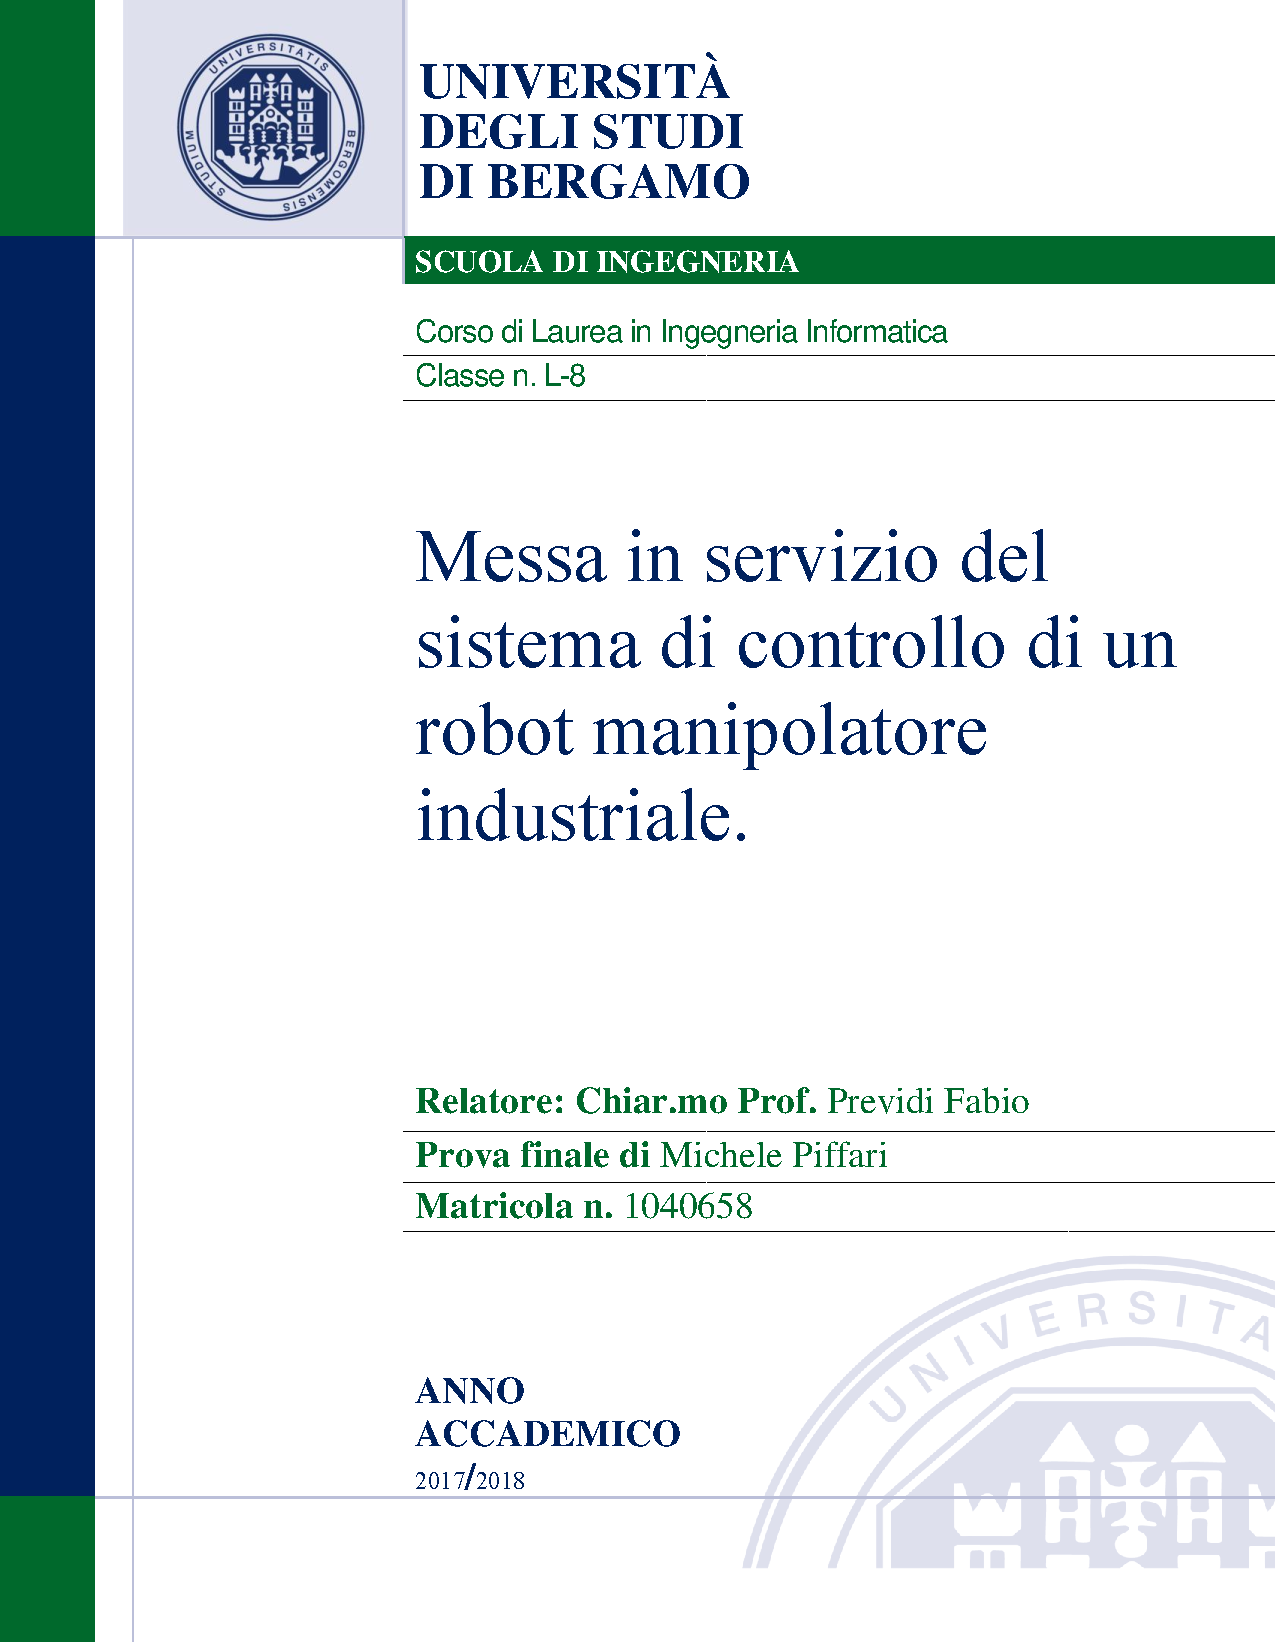
\includepdf[pages={1},pagecommand={\thispagestyle{empty}}]{fronteingegnerialt.pdf}
	%%============= DOCUMENTO ==========================================

	%====================================================================
	\thispagestyle{empty}
	\hfill
	\vfill
	\textsc{todo}
	Questo documento è stato rilasciato con licenza Creative Commons Attribuzione
	3.0 Unported (CC BY 3.0). Per leggere il testo integrale della licenza si può
	visitare il sito web \url{http://creativecommons.org/licenses/by/3.0/legalcode}
	o spedire una lettera a Creative Commons, 171 Second Street, Suite 300, San
	Francisco, California, 94105, USA. Il testo è anche disponibile in italiano, in
	formato ridotto, all'indirizzo web
	\url{http://creativecommons.org/licenses/by/3.0/deed.it}.
	
	La tesi è stata scritta in \LaTeX{} sul sistema operativo Windows 10, con
	l'editor di testo TeXstudio e grazie ai suggerimenti tipografici degli utenti
	del forum del \GuIT ed alla guida 
	\href{http://www.lorenzopantieri.net/LaTeX_files/ArteLaTeX.pdf}{"L'arte di scrivere con \LaTeX{}"}.
	
	È possibile scaricare l'intero codice sorgente di questo documento, compreso l'elenco delle immagine, all'URL
	\url{https://github.com/Piffo/SourceCode_BachelorDegree.git}.

%==================================================================% Includo un .tex esterno
	%\cleardoublepage
	\thispagestyle{empty}
	\begin {flushright}
		\null \vspace {\stretch {1}}
			\emph{"The more we do, the more we can do; the more busy we are, the more leisure we have"}\\William Hazlitt
		\vspace {\stretch {2}}\null
	\end {flushright}
	\tableofcontents
	\listoffigures
	\lstlistoflistings
	%====================================================================
	\fncymain 
	\mainmatter
	\chapter{Introduzione}
	%======================= DOCUMENTO ======================================
Questo progetto si inserisce all'interno del percorso di ricerca avviato dal laboratorio del CAL \emph{(Control systems and Automation Laboratory)} dell'Università degli studi di Bergamo, il cui obbiettivo è stato quello di creare e gestire un sistema autonomo di pick and place da inserire in ambiente agricolo.

Il fulcro dello studio condotto è stato quello di eseguire uno start up del sistema: in un primo momento si è andato a studiare la componentistica hardware, composta dal manipolatore \emph{ABB IRB 120} e dal controllore \emph{IRC5 Compact}, mettendo in atto un lavoro di \emph{unboxing} del sistema stesso, installando i collegamenti fisici tra il manipolatore e il controllore e cablando la connessione alla rete elettrica.

Dopo una prima fase appunto più pratica, che ha portato sostanzialmente alla cablatura del sistema unitamente ad un primo approccio al mondo della robotica (il cui report è contenuto nella parte~\vref{part:Il_sistema}), il focus del progetto si è spostato sulla parte di controllo e gestione della traiettoria del manipolatore: sono stati esaminati soprattutto la parte di comunicazione PC/Controller e la cinematica del braccio robotico, implementata poi, in via sperimentale e non definitiva, tramite software. Questa è proprio una peculiarità del mondo della robotica in cui si ha la necessità di focalizzarsi contemporaneamente sia sul design del robot (e quindi sulla geometria e sulle matrici caratterizzanti il movimento) sia sulla tipologia di utilizzo dello stesso robot da parte dell'utente finale. 

Saranno quindi qui riportate le analisi condotte sul sistema a livello hardware e lo studio del controllo dal punto di vista software, in una forma più manualistica, per poter aiutare eventuali progetti futuri riguardanti lo sviluppo di sistemi basati su questa famiglia di manipolatori \emph{ABB}, per mezzo dello studio della componentistica nella parte(parte~\vref{part:Il_sistema}) unitamente alle possibilità di controllo analizzate invece nella parte~\vref{part:Il_controllo}.

L'obbiettivo del progetto, chiudendo così la parte introduttiva, è quindi quello di andare a capire il funzionamento del manipolatore, studiandone la componente software \emph{ABB}, prodotta in RAPID: una volta consolidata la conoscenza del dominio applicativo "software" siamo andati poi a validare il modo migliore per poter governare il movimento del manipolatore stesso tramite PC, analizzando tutte le possibilità di comunicazione disponibili per poter fare dialogare il controllore \emph{IRC5 Compact} con il braccio \emph{ABB IRB 120}.
%========================================================================
	\label{chapter:introduction}
	\part{Il sistema}
	\label{part:Il_sistema}
	\chapter{Il manipolatore IRB 120}
	%================= DOCUMENTO =========================================
Il manipolatore ABB IRB 120 \emph{(Industrial Robot Base)} rappresenta una soluzione \emph{economica} e \emph{affidabile} per produzioni in grande quantità su linee di produzione automatizzate, con un investimento contenuto: si tratta perciò di una nuova frontiera di manipolatori industriali i quali, secondo la \emph{definizione \textsc{ISO}} \cite{ISO:normaRobot}, possono essere definiti come:
\begin{quoting}

\emph{"A robot is an automatically controlled, reprogrammable, multipurpose and manipulative machine with
	several reprogrammable axes, which may be either fixed in place or mobile for use in
	industrial automation applications"}
\end{quoting}

Il manipolatore industriale oggetto dello studio in questo progetto, come esplicitato precedentemente, è l'ABB IRB 120, il quale è il più piccolo robot industriale universale commercializzato da ABB (\emph{Asea Brown Boveri}), del peso di soli 25kg e con la possibilità di movimentare carichi fino a 3/4 kg per mezzo di uno sbraccio massimo di 580 \si{\milli\metre} \cite{ABB:Manul_irb120}.

Queste caratteristiche rendono IRB 120 il manipolatore più facilmente integrabile presente sul mercato: progettato con una leggera struttura in alluminio, nella quale i potenti motori compatti assicurano un rapido movimento del robot (velocità di avanzamento lineare massima di 6000 \si{\milli\metre}/\si{\second}) con elevata accelerazione pur mantenendo precisione, di circa \emph{risoluzione \ang{0.01}} e agilità in qualsiasi applicazione e tipologia di movimento.
 
\newpage
\section{Morfologia}
L'IRB 120 fa parte quindi della classe dei manipolatori industriali: dal punto di vista morfologico, esso presenta 6 gradi di libertà \emph{(numero di coordinate libere)}, ovvero la movimentazione del braccio stesso avviene per mezzo di 5 \emph{bracci (links)} collegati da 6 \emph{giunti (joints)}\label{text:joints} di tipo rotoidale come si può vedere in figura \vref{fig:IRB120img}.
\begin{figure}[h]
	\centering
	\subfloat[]{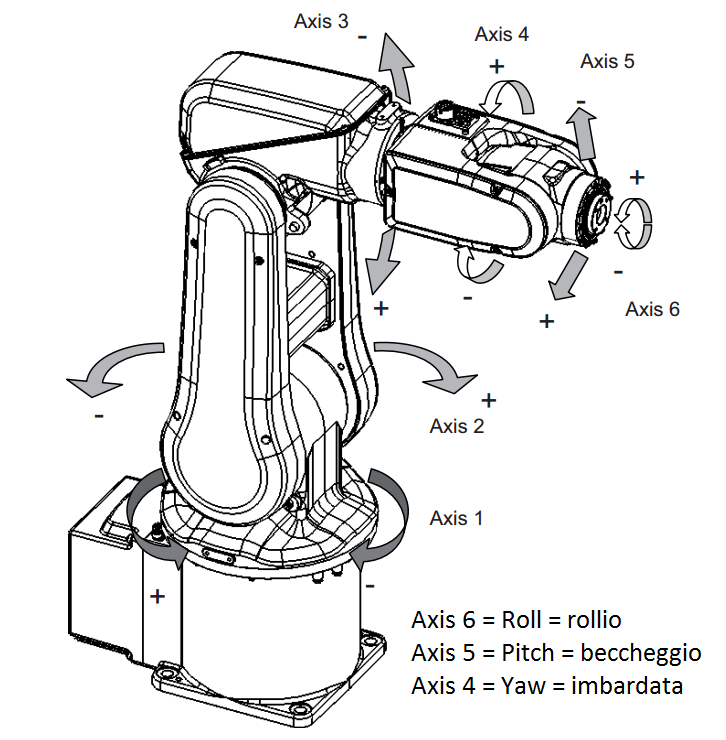
\includegraphics[width=0.55\textwidth]{Immagini/IRB120}}\quad
	\subfloat[]{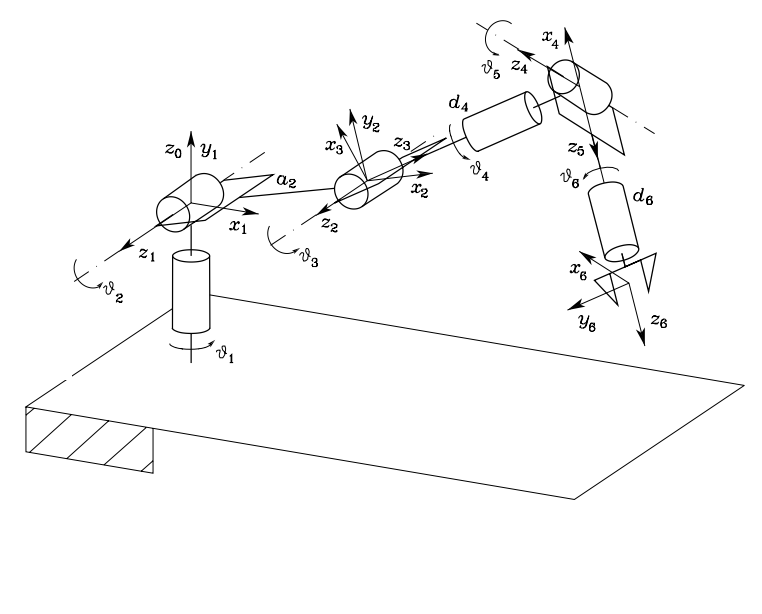
\includegraphics[width=0.55\textwidth]{Immagini/IRB120_Model}}
	\caption{Struttura fisica manipolatore ABB IRB120 \emph{(a)} e relativo modello matematico \emph{(b)}}
	\label{fig:IRB120img}
\end{figure}

Entrando più nel dettaglio, si intuisce facilmente come l'IRB 120 faccia parte della categoria dei manipolatori industriali antropomorfi: le presenza di 6 giunti rotazionali va a creare una forte somiglianza con quello che è il braccio umano.
\begin{figure}
	\centering
	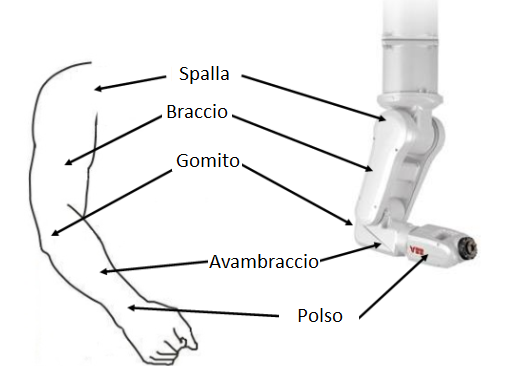
\includegraphics[width=0.5\textwidth]{Immagini/BraccioUmano_IRB120}
	\caption{Morfologia del manipolatore industriale in similitudine con la morfologia del braccio umano}
	\label{fig:HumanArmIRB120}
\end{figure}

Ovviamente il braccio umano, il quale presenta \emph{7 \textsc{DOF} (Degrees Of Freedom)}, ha una mobilità maggiore dovuta alla sua ridondanza: infatti il corpo umano è dotato di 2 braccia coordinate con 7 \textsc{DOF} ciascuno con mani con 18 \textsc{DOF} e flessibilità, il tutto coordinato da visione \cite{DOF:HumanArm}.

Nonostante ciò, 6 \textsc{dof} risultano essere sufficienti: infatti un corpo rigido nello spazio è univocamente determinato da 6 parametri, tre dei quali individuano la posizione \emph{(x,y,z)} e tre l'orientamento \emph{($\psi$,$\vartheta$,$\varphi$)}.

Traslando questi concetti teorici sul nostro manipolatore IRB 120, la posizione può essere gestita tramite i primi tre giunti, mentre l'orientamento viene gestito tramite gli ultimi tre giunti della catena cinematica (capitolo~\vref{sec:Kinematics}).
\section{Caratteristiche tecniche principali}
Nell'analisi della movimentazione del manipolatore IRB 120, si è rivelato necessario andare ad analizzare alcune delle caratteristiche fisiche principali, studiandone i limiti principali unitamente alla flessibilità che esse offrono.
\subsection{Intervalli di movimento}
%Creo una tabella in testo
\begin{center}
\label{tab:movIRB120}
\begin{tabular}{l|c|c}
	\toprule
	\textbf{Spostamento assi} & \textbf{Area di lavoro} & \textbf{Velocità massima} \\
	\midrule
	Asse 1 \emph{(Rotazione)} & $\ang{165}$ to $\ang{-165}$ & $\ang{250}/s$ \\
	Asse 2 \emph{(Braccio)} & $\ang{110}$ to $\ang{-110}$ & $\ang{250}/s$ \\
	Asse 3 \emph{(Braccio)} & $\ang{70}$ to $\ang{-90}$ & $\ang{250}/s$ \\
	Asse 4 \emph{(Polso)} &	$\ang{160}$ to $\ang{-160}$ & $\ang{320}/s$ \\ 
	Asse 5 \emph{(Brandeggio polso)} & $\ang{120}$ to $\ang{-120}$ & $\ang{320}/s$ \\
	Asse 6 \emph{(Rotazione polso)} & $\ang{400}$ to $\ang{-400}$ & $\ang{420}/s$ \\
	\bottomrule
\end{tabular}
\end{center}
\newpage
\subsection{Dimensioni fisiche}
\begin{figure}[h]
	\centering
	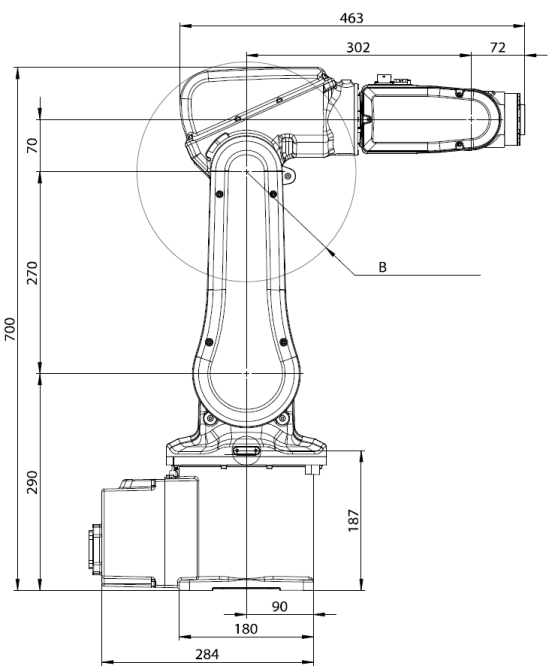
\includegraphics[width=0.5\textwidth]{Immagini/DimensioniManipolatore}
	\caption{Dimensioni fisiche espresse, in mm, dei bracci del manipolatore IRB 120}
	\label{fig:IRB120_Dimension}
\end{figure}
\subsection{Range di lavoro e raggio di curvatura}

In base a quelle che sono le dimensioni fisiche del manipolatore (figura~\vref{fig:IRB120_Dimension}) e le massime angolazioni raggiungibili singolarmente da ognuno dei 6 joint, il TCP (\emph{Tool Center Point} - \vref{item:TCP}) può raggiungere le seguenti zone di lavoro:
\begin{figure}[h]
	\centering
	\subfloat[]{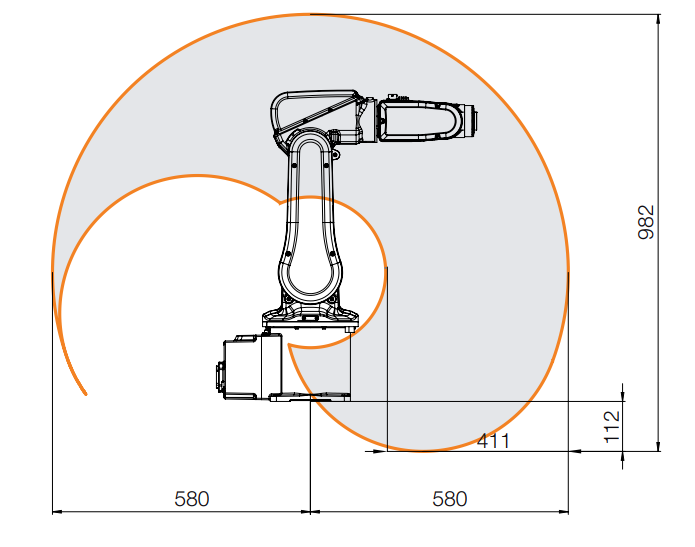
\includegraphics[width=0.45\textwidth]{Immagini/RangediLavoro}}\quad
	\subfloat[]{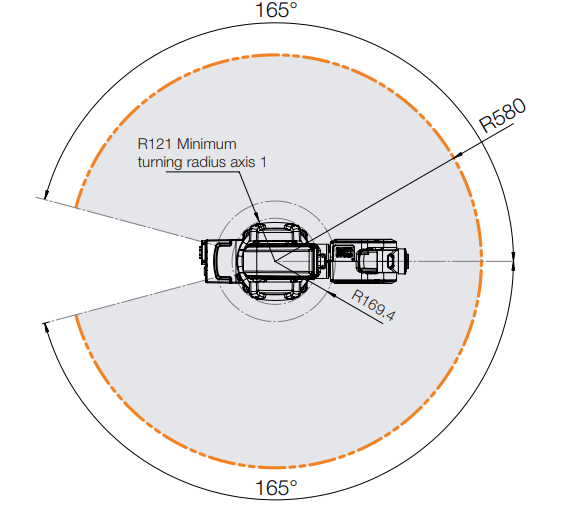
\includegraphics[width=0.45\textwidth]{Immagini/RaggiodiCurvatura}}
	\caption{Range di lavoro \emph{(a)} e raggio di curvatura \emph{(b)}}
	\label{fig:RangeFunzionamento}
\end{figure}
\subsection{Prestazioni}
\begin{center}
	\label{tab:prestazioniIRB120}
	\begin{tabular}{c|c}
		\toprule
		& \textbf{IRB 120} \\
		\midrule
		\textbf{Ciclo con 1kg di carico} & \\
		$25\times300\times25 \si{\milli\metre}$ & 0.58\si{\second} \\
		$25\times300\times25 \si{\milli\metre}$ con riorientamento \ang{180} asse 6 & 0.92\si{\second} \\
		Tempo di accelerazione$0-1\si{\metre}/\si{\second}$ & 0.07\si{\second} \\
		\bottomrule
	\end{tabular}
\end{center}
\section{La cinematica}
\label{sec:Kinematics}
%======================================================================
Per poter gestire e programmare la movimentazione del manipolatore ABB IRB 120 è necessario effettuare uno studio della sua cinematica (figura~\vref{fig:Cinematica_DirInv}), ovvero di quello che è il legame tra lo stato dei 6 giunti e la posizione e l'orientamento dell'end-effector: questo legame deve essere gestito in base a quelli che sono i sistemi di riferimento principali e le dimensioni geometriche riguardanti il manipolatore.

Analizzeremo innanzitutto quelli che sono i sistemi di coordinate utilizzati per definire la movimentazione del manipolatore ABB IRB 120, andando poi a sviluppare uno studio della cinematica diretta e inversa del manipolatore stesso, fornendo così gli strumenti necessari, a livello matematico, per definire con precisione le coordinate spaziali del robot.

\begin{figure}[h]
	\centering
	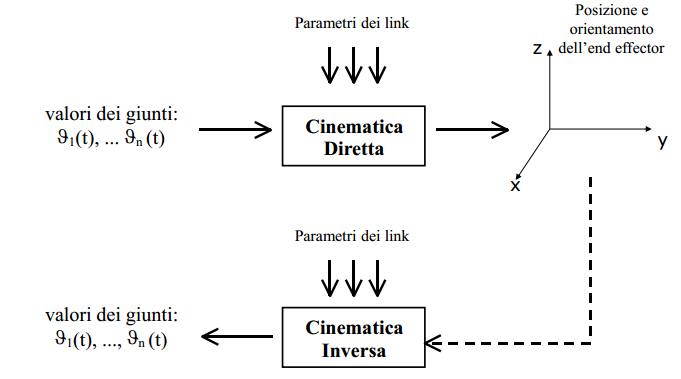
\includegraphics[width=0.7\textwidth]{Immagini/Cinematica_inv_dir_scheme}
	\caption{Cinematica diretta e inversa\cite{rep:Slide_Brugali1}}
	\label{fig:Cinematica_DirInv}
\end{figure}



\subsection{Sistemi di coordinate}

Come già ribadito in precedenza, quello che si vuole andare a gestire è la traiettoria del manipolatore, ovvero la posizione dell'end effector: questo però è possibile solo dal momento in cui si definisce un punto di riferimento rispetto al quale si riferisce il moto, ovvero definendo un origine dalla quale si sviluppa poi un sistema di coordinate bi o tridimensionale. 

Nell'ambiente di sviluppo RobotStudio (capitolo~\vref{text:RobotStudio}) si lavora con più sistemi di riferimento, permettendo la creazione di aree di lavoro complesse; questi specifici sistemi di coordinate, che permettono una gestione del moto nell'area di lavoro più articolata, semplificando nello stesso tempo la programmazione fuori linea, sono:
\begin{figure}[h]
	\centering
	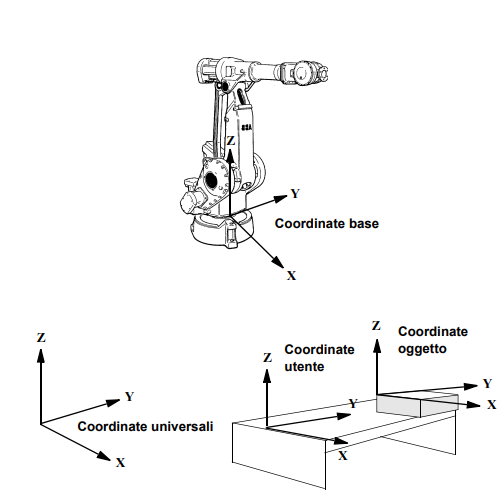
\includegraphics[width=0.7\textwidth]{Immagini/SistemiDiCoordinate}
	\caption{Sistemi di riferimento esterni per la gestione della traiettoria del manipolatore}
	\label{fig:SdR}
\end{figure}
\begin{description}
	\item[Sistema di coordinate universale:] definito anche WCS \emph{(World Coordinate System)}, definisce un riferimento rispetto al pavimento o alla cella di lavoro, che rappresenta il punto di partenza per gli altri sistemi di coordinate. Utilizzando questo sistema di coordinate, è possibile mettere in relazione la posizione del robot con un	punto fisso in fabbrica, per esempio. 
	Risulta quindi essere molto utile quando due robot lavorano insieme, dovendo collaborare tra di loro.
	
	\item[Sistema di coordinate della base:] esso ha come origine il punto centrale alla base del robot, ovvero la base d'appoggio del robot.
	
	\item[Sistema di coordinate dell'utente:] esso specifica la posizione di un'attrezzatura esterna, fornendo così la possibilità di inserire sistemi di	coordinate 	per diversi attrezzi e/o superfici di lavoro. 
	
	\item[Sistema di coordinate dell'oggetto di lavoro:] in sistemi di lavoro, anche di media complessità, un attrezzo potrebbe includere vari oggetti di lavoro che devono essere elaborati o gestiti dal robot.	
	Questo	consente di definire un sistema di coordinate per ogni oggetto (si possono quindi avere più sistemi di coordinate di questo tipo) per poter regolare
	più facilmente il programma nel caso in cui un oggetto venga spostato oppure un
	nuovo elemento, simile a quello precedente, debba essere programmato in una diversa posizione, permettendo una ridefinizione automatica della traiettoria. 
	
	Esso viene ad essere posizionato rispetto al sistema di coordinate utente, riuscendo ad adattarsi perfettamente alla programmazione off-line, in quanto le posizioni specificate	possono essere ricavate direttamente da un disegno del work object, ovvero dell'area di lavoro (detta alternativamente anche workstation).
	\item[Sistema di coordinate del polso:]\label{item:SdR_Polso} esso rappresenta il sistema di riferimento del giunto numero 6; in sostanza, come per gli altri 5 assi, esso permette di definire la posizione del centro del giunto stesso. Merita una menzione particolare poichè questo sistema di riferimento definisce l'orientamento del manipolatore (figura~\vref{fig:axis6}).
	\begin{figure}[h]
		\centering
		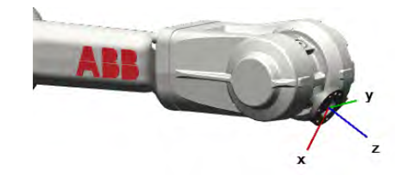
\includegraphics[width=0.5\textwidth]{Immagini/SistemaDiRiferimento_Polso}
		\caption{Sistema di coordinate polso}
		\label{fig:axis6}
	\end{figure}
	\item[Sistema di coordinate dell'utensile di lavoro:]\label{item:TCP} esso permette di definire la posizione e l'orientamento dell'utensile agganciato al polso. Spesso chiamato TCP \emph{(Tool Center Point)} la sua importanza è quindi estrema, poichè permette di gestire il punto con il quale il manipolatore andrà ad agire direttamente sull'oggetto, definendone la gestione della lavorazione/manipolazione richiesta (figura~\vref{fig:TCP})
\end{description}
\begin{figure}[h]
	\centering
	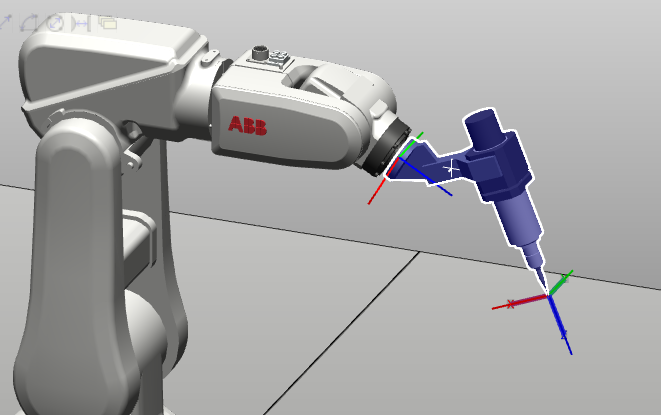
\includegraphics[width=0.5\textwidth]{Immagini/TCP}
	\caption{Tool Center Point}
	\label{fig:TCP}
\end{figure}
Da queste brevi descrizioni si capisce come la gestione della traiettoria del manipolatore debba occuparsi della posizione e dell'orientamento del \emph{TCP} rispetto al sistema di riferimento oggetto: entrambi risultano essere definiti, a loro volta, rispetto al sistema di coordinate universale.



\subsection{Descrizione di posizione e orientamento di un sistema di riferimento}
Come si può vedere in figura~\vref{fig:Catena_Cinematica}, l'ABB IRB 120 può essere modellizzato come un insieme di sistemi di riferimento: trattandosi infatti di un manipolatore robotico, esso è costituito da una sequenza di organi meccanici \emph{(links)}, collegati tra loro da \emph{joints}, i quali permettono di individuare così una catena cinematica aperta, per l'assenza di anelli chiusi.
\begin{figure}[h]
	\centering
	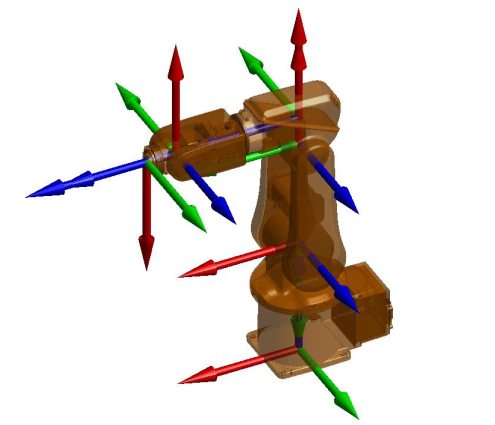
\includegraphics[width=0.6\textwidth]{Immagini/CatenaCinematica}
	\caption{Catena cinematica IRB 120}
	\label{fig:Catena_Cinematica}
\end{figure}

Ad ogni link è associato un sistema di coordinate che ne caratterizza la posizione: quindi il fulcro del problema cinematico si riduce alla definizione della posizione e dell'orientamento di un generico sistema di riferimento, sfruttando poi le caratteristiche della catena cinematica (figura~\vref{fig:Catena_Cinematica}) per andare a posizionare il robot.

La posizione di un sistema di riferimento è banalmente individuata dalle coordinate $x,y,z$ della sua origine, sempre riferite ad un sistema fissato: ciò che comporta uno studio più approfondito è l'orientamento di una terna rispetto ad un'altra, possibile andando ad utilizzare i versori della prima terna rispetto a quelli della seconda (figura~\vref{fig:Rotazione_SistemaDiRiferimento}).
\newpage
\subsubsection{Rotazioni elementari}
\label{subsub:Rot_elementari}
\begin{figure}[h]
	\centering
	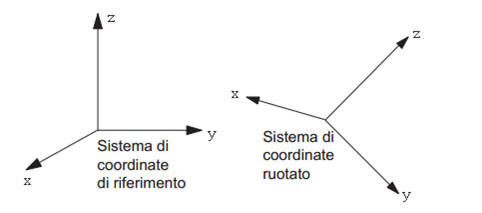
\includegraphics[width=0.6\textwidth]{Immagini/Rotazione_SistemiDiRiferimento}
	\caption{Rotazione di una terna rispetto ad un'altra}
	\label{fig:Rotazione_SistemaDiRiferimento}
\end{figure}
 Riferendosi alla figura~\vref{fig:Rotazione_SistemaDiRiferimento}, andando a far coincidere le origini delle due terne, ovvero operando una traslazione della seconda terna rispetto alle prima, possiamo vedere i versori dei tre assi traslati come tre vettori separati, i quali possono quindi essere espressi rispettivamente come:
 \begin{itemize}
 	\item $\hat{\vec{x}}= $ versore dell'asse $ x=(x_1,x_2,x_3)\Rightarrow$ Il versore direzionale dell'asse x  presenta una componente $x_1$ lungo l'asse x del sistema di riferimento considerabile \emph{fisso}, $x_2$ lungo y e $x_3$ lungo z.
 	\item $\hat{\vec{y}}=$ versore dell'asse $y=(y_1,y_2,y_3)\Rightarrow$ Il versore direzionale dell'asse y  presenta una componente $y_1$ lungo l'asse x del sistema di riferimento considerabile \emph{fisso}, $y_2$ lungo y e $y_3$ lungo z.
 	\item $\hat{\vec{z}}=$versore dell'asse z$=(z_1,z_2,z_3)\Rightarrow$ Il versore direzionale dell'asse z  presenta una componente $z_1$ lungo l'asse x del sistema di riferimento considerabile \emph{fisso}, $z_2$ lungo y e $z_3$ lungo z.
 \end{itemize}
La matrice di rotazione prende quindi la seguente forma: il pedice posto alla sinistra dellla matrice indica il sistema di riferimento descritto, mentre l'apice indica il riferimento usato per la descrizione, ovvero la matrice \textbf{R} (matrice~\vref{mat:RotationMatrix}) indica la matrice di rotazione che descrive la terna $\{$B$\}$ rispetto alla terna $\{$A$\}$.
\begin{equation}
	\label{mat:RotationMatrix}	
	\textbf{$\prescript{A}{B}{\textsc{R}}$}=
	\begin{bmatrix}
	x_1&y_1&z_1\\
	x_2&y_2&z_2\\	
	x_3&y_3&z_3
	\end{bmatrix}
	=
	\begin{bmatrix}
	\hat{\vec{x_B}}\cdot\hat{\vec{x_A}}&\hat{\vec{y_B}}\cdot\hat{\vec{x_A}}&\hat{\vec{z_B}}\cdot\hat{\vec{x_A}}\\
	\hat{\vec{x_B}}\cdot\hat{\vec{y_A}}&\hat{\vec{y_B}}\cdot\hat{\vec{y_A}}&\hat{\vec{z_B}}\cdot\hat{\vec{y_A}}\\	
	\hat{\vec{x_B}}\cdot\hat{\vec{z_A}}&\hat{\vec{y_B}}\cdot\hat{\vec{z_A}}&\hat{\vec{z_B}}\cdot\hat{\vec{z_A}}
	\end{bmatrix}
\end{equation}
La matrice~\vref{mat:RotationMatrix} è detta anche matrice dei coseni direttori dato che, per definizione di prodotto vettoriale ($\hat{\vec{x_B}}\cdot\hat{\vec{x_A}}=\parallel\hat{\vec{x_B}}\parallel\cdot\parallel\hat{\vec{x_A}}\parallel\cdot\cos \alpha=\cos\alpha$), i componenti della matrice di rotazione saranno solamente dei coseni degli angoli compresi tra i versori.
\begin{figure}
	\centering
	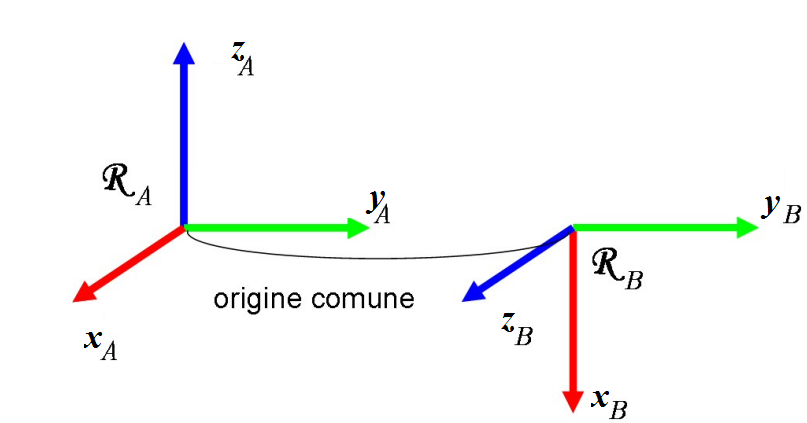
\includegraphics[width=0.5\textwidth]{Immagini/EsempioRotazione}
	\caption{Semplice esempio di rotazione di sistemi di riferimento}
	\label{fig:ShortExampleRotationMatrix}
\end{figure}
\newpage
Per poter trovare la semplice matrice di rotazione che descrive la rotazione in figura~\vref{fig:ShortExampleRotationMatrix}, le due possibilità che si hanno sono quelle di
\begin{itemize}
	\item  individuare i versori del sistema di riferimento B rispetto al sistema A.
	\item sviluppare i prodotti vettori (ricordando che esso si annulla per vettori ortogonali tra di loro).
\end{itemize} 
Detto ciò possiamo trovare la matrice come:
\begin{equation}
	\vec{x_B}=
	\begin{bmatrix}
		0\\	
		0\\
		-1
	\end{bmatrix}
	,
	\vec{y_B}=
	\begin{bmatrix}
		0\\	
		1\\
		0
	\end{bmatrix}
	,
	\vec{z_B}=
	\begin{bmatrix}
		1\\	
		0\\
		0
	\end{bmatrix}
\end{equation}
La matrice di rotazione della figura~\vref{fig:ShortExampleRotationMatrix} sarà quindi:
\begin{equation}
	\label{mat:ExampleRotationMatrix}	
	\textbf{$\prescript{A}{B}{\textsc{R}}$}=
	\begin{bmatrix}
	0&0&0\\
	0&1&0\\	
	-1&0&1
	\end{bmatrix}
\end{equation}
Quelle considerate finora, tramite semplici esempi, rappresentano rotazioni elementari (figura~\vref{fig:RotazioniElementari}), ovvero che avvengono lungo un determinato asse.
Andando ad applicare quanto di semplice fatto nell'esempio in figura~\vref{fig:ShortExampleRotationMatrix}, siamo in grado di andare a trovare le matrici di rotazione per i casi di rotazioni generiche:
\begin{description}
	\item[$\bullet$ Rotazione intorno asse x di angolo $\gamma$: ] \begin{equation}
		\label{mat:RotationMatrix_x}	
		\textbf{$\textsc{R}_X(\gamma)$}=
		\begin{bmatrix}
			1&0&0\\
			0&\cos \gamma&-\sin \gamma\\
			0&\sin \gamma&\cos \gamma
		\end{bmatrix}
	\end{equation}
	\item[$\bullet$ Rotazione intorno asse y di angolo $\beta$: ] \begin{equation}
		\label{mat:RotationMatrix_y}	
		\textbf{$\textsc{R}_y(\beta)$}=
		\begin{bmatrix}
			\cos \beta&0&\sin \beta\\
			0&1&0\\
			-\sin \beta&0&\cos \beta
		\end{bmatrix}
	\end{equation}
	\item[$\bullet$ Rotazione intorno asse z di angolo $\alpha$: ] \begin{equation}
		\label{mat:RotationMatrix_z}	
		\textbf{$\textsc{R}_z(\alpha)$}=
		\begin{bmatrix}
			\cos \alpha&-\sin \alpha&0\\
			\sin \alpha&\cos \alpha&0\\	
			0&0&1
		\end{bmatrix}
	\end{equation} 
\end{description}
\begin{figure}
	\centering
	\subfloat[][Rotazione intorno a x]{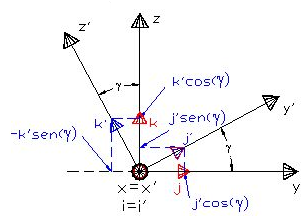
\includegraphics[width=0.40\textwidth]{Immagini/Rot_asse_x}}
	\subfloat[][Rotazione intorno a y]{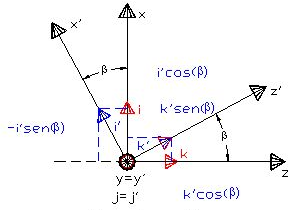
\includegraphics[width=0.40\textwidth]{Immagini/Rot_asse_y}}\\
	\subfloat[][Rotazione intorno a z]{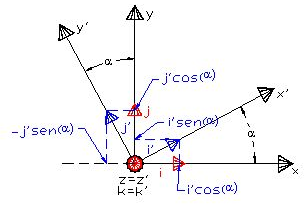
\includegraphics[width=0.40\textwidth]{Immagini/Rot_asse_z}}	
	\caption{Rotazioni elementari}
	%[Immagine presa dal sito http://slideplayer.it/slide/537558/ in data 03/03/18] 
	\label{fig:RotazioniElementari}
\end{figure}

\subsubsection{Composizione delle matrici di rotazione: rotazioni complesse}
\label{subsubsection:RotComplex}
Concetto importante, che poi riapparirà, seppur se in forma più complessa, nella convenzione di Denavit-Hartenberg (sottosezione~\vref{subsubsection:D-H}), è quello di \emph{composizione delle matrici di rotazione}.

Finora sono state analizzate solamente rotazioni di tipo elementare, ovvero che avvengo intorno ad un unico asse: ogni altra rotazione, e la corrispondente matrice, possono essere ottenuti combinando opportunamente le rotazioni elementari.

\label{text:ComposizioneRotazioni}Si tratta quindi di scomporre la rotazione complessiva in tante rotazioni elementari: la matrice complessa è sempre ottenibile dal prodotto delle matrici di rotazioni associate alle singole sotto rotazioni "sequenziali" che possono essere effettuate in 
\begin{itemize}
	\item Terna fissa: la rotazione avviene sempre intorno agli assi del sistema di riferimento "iniziale", che viene mantenuto fisso e costante durante tutte le rotazioni sequenziali.
	\item Terna mobile: in questo caso la rotazione viene eseguita rispetto al sistema di coordinate ottenuto dalla precedente rotazione.
\end{itemize}
\begin{figure}
	\centering
	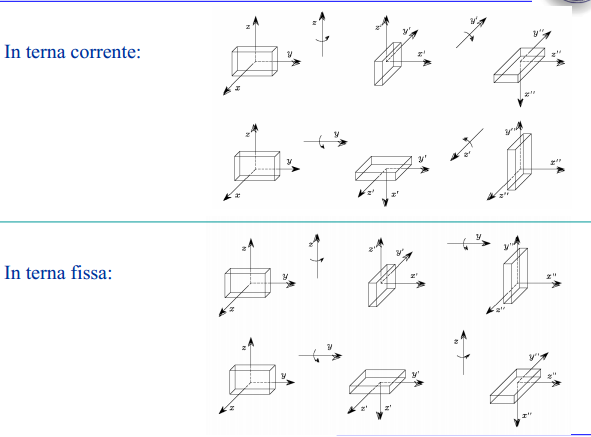
\includegraphics[width=0.75\textwidth]{Immagini/Rot_TernaFissaMobile}
	\caption{Composizione di rotazioni in terna fissa e mobile \cite{book:RobotIndustriali}}
	\label{fig:Rot_TernaFissa_Mobile}
\end{figure}
Il concetto importante è però che, indipendentemente dal tipo di rotazione composta che si va a considerare (se rispetto ad una terna fissa oppure mobile), per poter descrivere rotazioni complesse è sufficiente effettuare una moltiplicazione matriciale tra le matrici di rotazione di ogni singolo orientamento elementare.

Per esempio, supponendo di avere tre terne A, B e C diversamente orientate, si può individuare la matrice di rotazione che esprime l'orientamento della terna C rispetto ad A ($\prescript{A}{C}{\textsc{R}}$) con una moltiplicazione matriciale di questo tipo
\begin{equation}
	\prescript{A}{C}{\textsc{R}}=\prescript{A}{B}{\textsc{R}} \prescript{B}{C}{\textsc{R}}
\end{equation}
Va da se che, unendo le informazioni in merito a posizione e rotazione di un sistema di riferimento, si è in grado di individuare in maniera univoca una terna mobile rispetto ad una fissa. 

Tipicamente tale descrizione reciproca tra terne è espressa mediante una singola matrice che comprende sia le informazioni di posizione che di orientamento, la quale prende il nome di \emph{matrice di trasformazione omogenea} ed è così definita
\begin{equation*}
	\label{equation:MatrixOmogenous}
	\left[
	\begin{array}{l|r}
		\prescript{A}{B}{\textsc{R}}&pos\ped{B,A}\\ \hline
		\vec{0} & \vec{1}
	\end{array}
	\right]
\end{equation*}



\newpage
\subsection{Cinematica diretta IRB 120}

Il problema cinematico diretto si impone a di trovare il posizionamento dell'end-effector dato il valore dei giunti del manipolatore: nello specifico l'IRB 120 fa parte della categoria dei bracci seriali, ovvero di quei manipolatori costituiti da una catena cinematica aperta, composti da una sola sequenza di \emph{link} che connette i due estremi del robot stesso.
\begin{figure}[h]
	\centering
	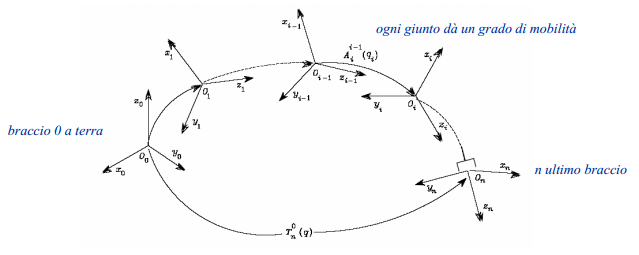
\includegraphics[width=0.75\textwidth]{Immagini/CatenaCinematicaOpen_Example}
	\caption{Esempio di catena cinematica aperta formata da \emph{n} bracci \cite{book:RobotIndustriali}} 
	\label{fig:CatenaCinematicaOpen}
\end{figure}
La risoluzione della cinematica diretta dell'IRB 120 è concettualmente molto semplice: si tratta di applicare una composizione di rotazioni in terna fissa a sistemi di riferimento solidali ad ognuno dei 6 bracci, partendo dalla terna base, ed ottenendo così orientamento e posizione dall'ultima terna della catena (end-effector) espressa rispetto alla base del manipolatore.

La composizione di rotazioni analizzata nella sottosezione~\vref{text:ComposizioneRotazioni} era riferita alle sole matrici di rotazioni, le quali individuano esclusivamente informazioni in merito all'orientamento. Questo concetto, basato su moltiplicazioni matriciali, è però applicabile anche alle matrici di trasformazione omogenea, la cui forma è leggermente più complessa (data la presenza delle informazioni in merito alla posizioni come si vede nel paragrafo~\vref{equation:MatrixOmogenous}).

Il procedimento è quindi si molto semplice: ma esiste una qualche convenzione per fissare le terne solidali ad ogni giunto (sezione ~\vref{text:joints}) in modo sistematico per facilitare la risoluzione dei prodotti matriciali?

\subsubsection{Metodo di Denavit-Hartenberg}\label{subsubsection:D-H}
Un possibile modo per poter trovare le 6 terne solidali ad ognuno degli altrettanti 6 giunti è quello di andare a posizionarle secondo il metodo di Denavit-Hartenberg: in questa sede non entreremo nei dettagli di quello che è l'algoritmo iterativo per individuare e definire la terna solidale ad ognuno dei giunti rispetto al precedente, ma ci limiteremo a rappresentarne gli aspetti più importanti e le conseguenze principali.
\newpage
La scelta dei sistemi di riferimento solidali per ogni giunto è basata quindi su due "algoritmi" iterativi:
\begin{itemize}
	\item \emph{Numerazione dei bracci e dei giunti:} ogni braccio (\emph{link}) viene numerato da 0 a \emph{n} a partire dalla base e arrivando all'organo terminale; ognuno di essi sarà individuato dai simboli $L_0,L_1,\dots,L_n$. Un manipolatore seriale, come l'IRB 120 (significa che è rappresentabile tramite una \emph{catena cinematica aperta}) con \emph{n} bracci, avrà $n-1$ giunti, designati $J_1,J_2,\dots,J_n$, dove il giunto $J_i$ collega i bracci $L\ped{i-1}$ e $L_i$.
	\item \emph{Assegnazione degli assi z dei sistemi di riferimento:} al membro \emph{i-}esimo ($0\le\emph{i}\le\emph{n}$) si associa un sistema di riferimento solidale $\{O^i,x^i,y^i,z^i\}$ il cui asse $z^i$ coincide con l'asse del giunto $J\ped{i+1}$, cioè con il giunto a valle. Come si osserva nella figura~\vref{fig:AssiZ_DH}, gli assi z dei bracci $i-1$ e $i$ hanno la stessa direzione degli assi z rispettivamente dei giunti $i$ e $i+1$.
\end{itemize}

\begin{figure}
	\centering
	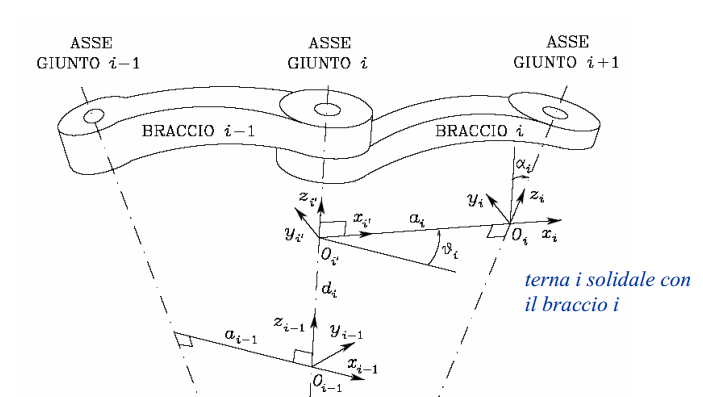
\includegraphics[width=0.75\textwidth]{Immagini/AsseZ_DH}
	\caption{Posizionamento sistemi di riferimento solidale per due bracci qualisiasi} 
	\label{fig:AssiZ_DH}
\end{figure}
Una volta assegnati gli assi $z_i$, possiamo andare a individuare:
\begin{itemize}
	\item \textsc{$O_i$}: l'origine del sistema di riferimento $i$-esimo è all'intersezione dell'asse $z_i$ con la normale comune. 
	(definibile come il segmento ortogonale agli assi del giunto $i$-esimo e di quello $i+1$-esimo, come si può vedere nella figura ~\vref{fig:AssiZ_DH}); si indica con $O^{'}_{i}$ l'intersezione della normale comune con $z\ped{i-1}$.
	\item \textsc{$x_i$}: è diretto lungo la normale comune agli assi $z_i$ e $z\ped{i-1}$, con verso positivo dal giunto $i$ al giunto $i+1$
	\item \textsc{$y_i$}: completa la terna destrorsa.	
\end{itemize}
\newpage
Da questi passi iterabili, per individuare i sistemi solidali ad ogni braccio, possiamo andare ad individuare quelli che sono i \emph{parametri di Denavit-Hartenberg}, che ci permettono di definire ogni terna rispetto alla precedente:
\begin{itemize}
 	\item \textsc{$a_i$}: distanza di $O_i$ da $O^{'}_{i}$, ovvero tra l'asse di giunto $i$-esimo e l'asse $(i+1)$-esimo.
	\item \textsc{$d_i$}: coordinata su $z\ped{i-1}$ di $O_i$.
	\item \textsc{$\alpha_i$}: angolo intorno all'asse $x_i$ tra l'asse $z\ped{i-1}$ e l'asse $z_i$, valutato positivo in senso antiorario; esso individua l'anngolo esistente tra l'asse di giunto $i$-esimo e l'asse $(i+1)$-esimo.
	\item \textsc{$\theta_i$}: angolo intorno all'asse $z\ped{i-1}$ tra l'asse $x\ped{i-1}$ e l'asse $x_i$ valutato positivo in senso antiorario	(detta anche \emph{variabile di giunto} nel caso di giunti rotoidali come nei manipolatori antropomorfi).
\end{itemize}
Quelli sopraelencati rappresentano i parametri cinematici, fondamentali per la risoluzione della cinematica (sia diretta che inversa) di un generico manipolatore.

Per il manipolatore IRB 120 in esame, questi parametri sono riportati all'interno della tabella sottostante (si noti il legame dei parametri cinematici di braccio con la figura~\vref{fig:IRB120_Dimension}):
\begin{table}[h]
	\caption{Parametri di Denavit-Hartenberg del manipolatore IRB 120}
	\centering
	\footnotesize
	\makebox[\columnwidth][c]{%
	\begin{tabular}{ccccc}
		\toprule
		\label{tab:DH_Parameters}
		\multirow{4}*{\textbf{Braccio i-esimo}}&\multicolumn{2}{c}{\textbf{Parametri cinematici di braccio}} & \multicolumn{2}{c}{\textbf{Parametri cinematici di giunto}} \\
		\cmidrule(lr){2-5}
		&Lunghezza di braccio  & Torsione di braccio  & Scostamento di giunto  & Angolo di giunto \\
		&(\textbf{a\ped{i}})&(\textbf{$\alpha$\ped{i}})&(\textbf{d\ped{i}})&(\textbf{$\theta$\ped{i}})\\
		\midrule
		1 & 0   & \ang{-90} & 290 & $\theta_1$\\ 
		2 & 270 & \ang{0}   &   0 & $\theta_2-\ang{90}$\\
		3 & 70  & \ang{-90} &   0 & $\theta_3$\\
		4 & 0   & \ang{90}  & 302 & $\theta_4$\\
		5 & 0   & \ang{-90} &   0 & $\theta_5$\\
		6 & 0   & \ang{0}   &  72 & $\theta_6+\ang{180}$
	\end{tabular}}	
\end{table}
\begin{figure}
	\centering
	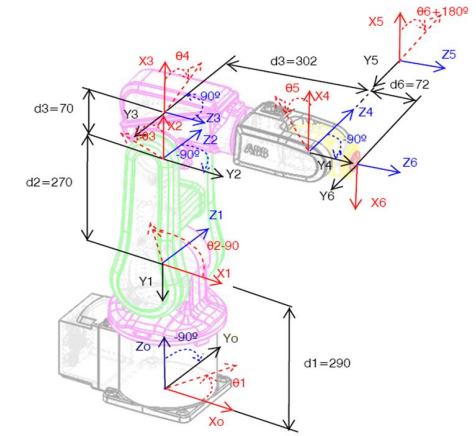
\includegraphics[width=0.75\textwidth]{Immagini/Parametri_DH}
	\caption{Rappresentazione dei parametri di Denavit-Hartenberg} 
	\label{fig:Rappresentazione_DH_Param}
\end{figure}

I parametri nella tabella \ref{tab:DH_Parameters} permettono di andare a rappresentare la matrice di trasformazione generica di un braccio: la matrice~\vref{mat:DH_4MatrixMoltiplication} permette di descrivere la trasformazione che il braccio (\emph{link}) introduce sui due giunti che si trovano alla sua estremità.

Per ricavare invece la matrice di trasformazione omogenea  
$\prescript{i-1}{i}{\textsc{T(q\ped{i})}}$, si vanno ad aggiungere tre terne ausiliarie $\{P\}$,$\{Q\}$ ed $\{R\}$, andando a scrivere le matrici di rotazioni che descrivono ciascuna di essa rispetto a quella precedente (computazione omessa in questa sede).

Andando poi a sfruttare la teoria della composizione di matrici di rotazione  (valida anche per le matrici di trasformazione omogenee viste nella sezione~\vref{equation:MatrixOmogenous}) possiamo scrivere la matrice che descrive la terna $\{i\}$ rispetto alla terna $\{i-1\}$ attraverso la composizione delle quattro matrici di trasformazione relative agli altrettanti sistemi di riferimento: si tratta di andare a moltiplicare in sequenza, una matrice omogenea che descrive una rotazione, due matrici omogenee che rappresentano altrettante traslazioni ed infine un'altra matrice rappresentate rotazione ottenendo il seguente risultato
\begin{equation}
	\footnotesize
	\label{mat:DH_4MatrixMoltiplication}
	\prescript{i-1}{i}{T}	= \prescript{Q}{R}{T} \prescript{R}{i}{T} \prescript{P}{Q}{T} \prescript{i-1}{P}{T}  =
	\begin{bmatrix}
		\begin{array}{ccc|c}
			\begin{matrix}
				\cos \ped{\theta_i}\\
				\sin \ped{\theta_i}\\	
				0
			\end{matrix}
			& 
			\begin{matrix}
				-\sin \ped{\theta_i} \cos \ped{\alpha\ped{i}}\\
				\cos\ped{\theta_i} \cos \ped{\alpha\ped{i}}\\	
				\sin \ped{\alpha\ped{i}}
			\end{matrix}
			&
			\begin{matrix}
				\sin \ped{\theta_i} \sin\ped{\alpha\ped{i}}\\
				-\sin \ped{\alpha\ped{i}}\\	
				\cos \ped{\alpha\ped{i}}
			\end{matrix}
			&
			\begin{matrix}
				a\ped{i} \cos \ped{\theta_i}\\
				a\ped{i} \sin \ped{\theta{i}}\\
				d_i
			\end{matrix}
			\\
			\hline
			0 & 0 & 0 & 1
		\end{array}
	\end{bmatrix}
\end{equation}

Quanto detto finora rappresenta la via risolutiva per risolvere la cinematica diretta del manipolatore in esame: andando ad analizzare ogni singola matrice di trasformazione $i-esima$ possiamo evidenziare ed isolare i seguenti passaggi (con la scritta $s_i$ si indica il valore $\cos \theta_{i}$ e con $s_i$ si rappresenta invece il $\sin\theta_{i}$). 
\begin{equation*}
	\prescript{0}{1}{T}	= A_1 =
	\begin{bmatrix}
		c_1 & 0    &-s_1& 0\\
		s_1 & 0    &c_1 & 0\\
		0   & -1   & 0  & 290\\
		0   & 0    &  0 & 1
	\end{bmatrix}
\end{equation*}\\

\begin{equation*}
	\prescript{1}{2}{T}	= A_2
	\begin{bmatrix}
		c_2 &-s_2 &  0 & 270c_2\\
		s_2 & c_2 &  1 & 270s_2\\
		0   & 0   &  1 & 0\\
		0   & 0   &  0 & 1
	\end{bmatrix}
\end{equation*}\\

\begin{equation*}
	\prescript{2}{3}{T}	= A_3
	\begin{bmatrix}
		c_3 & 0    &-s_3& 70c_3\\
		s_3 & 0    & c_3& 70s_3\\
		0   & -1   & 0  & 0\\
		0   & 0    & 0 & 1
	\end{bmatrix}
\end{equation*}\\

\begin{equation*}
	\prescript{3}{4}{T}	= A_4
	\begin{bmatrix}
		c_4 & 0    &s_4 & 0\\
		s_4 & 0    &-c_4& 0\\
		0   & 1    & 0  & 302\\
		0   & 0    & 0  & 1
	\end{bmatrix}
\end{equation*}

\begin{equation*}
	\prescript{4}{5}{T}	= A_5
	\begin{bmatrix}
		c_5 & 0    &-s_5& 0\\
		s_5 & 0    &c_5 & 0\\
		0   & -1   & 0  & 0\\
		0   & 0    & 0  & 1
	\end{bmatrix}
\end{equation*}

\begin{equation*}
	\prescript{5}{6}{T}	= A_6
	\begin{bmatrix}
		c_6 & -s_6 & 0  & 0\\
		s_6 & c_6  & 0  & 0\\
		0   & 0    & 1  & 72\\
		0   & 0    & 0  & 1
	\end{bmatrix}
\end{equation*}

L'ultimo step per poter giungere così alla risoluzione del problema cinematico diretto per il manipolatore IRB 120 è quello di andare a comporre le informazioni in merito alle roto-traslazioni di ogni sistema di riferimento, partendo dalla base e giungendo fino all'end-effector, ottenendo così posizione e orientamento dello stesso (per non appesantire ulteriormente il discorso, il risultato viene espresso in forma compatta).
\begin{figure}[h]
	\label{fig:Sol_DirectKin}
	\begin{equation*}
		\prescript{0}{6}{T}	= \prescript{0}{1}{T} \prescript{1}{2}{T} \prescript{2}{3}{T} \prescript{3}{4}{T} \prescript{4}{5}{T} \prescript{5}{6}{T}  = A_1A_2A_3A_4A_5A_6
		\begin{bmatrix}
			R_{11} & R_{12} & R_{13} & P_x\\
			R_{21} & R_{22} & R_{23} & P_y\\
			R_{31} & R_{32} & R_{33} & P_z\\
			0    & 0    & 0    & 1
		\end{bmatrix}
	\end{equation*}	
	\caption{Soluzione cinematica diretta manipolatore ABB IRB 120}
\end{figure}

\subsection{Cinematica inversa IRB 120}
Come visto nella matrice in figura~\vref{fig:Sol_DirectKin}, il problema cinematico diretto è sempre risolvibile attraverso la valutazione della matrice di trasformazione omogenea  $\prescript{0}{6}{T}$.

Il problema inverso invece, risulta essere più complicato: infatti, in base alla posizione spaziale fornita tramite coordinate $(x,y,z)$, ci possono essere casi in cui vi è un'unica soluzione, altri in cui ve ne possono essere multiple e altri ancora in cui non vi è alcuna possibile soluzione (quando per esempio la coordinata che si chiede di raggiungere si trova fuori dal range di azione del manipolatore stesso).

Non è quindi garantita nè l'esistenza nè l'unicità della soluzione della cinematica inversa e, nel caso ci siano più soluzioni possibili, si cerca di scegliere la migliore, andando a minimizzare i movimenti dei giunti.

Uno dei più intuitivi modi per poter risolvere il problema cinematico inverso, è quello di andare ad eguagliare la matrice di trasformazione dell'end-effector, che ne indica posizione ed orientamento rispetto alla base, con la sua espressione simbolica, ovvero la matrice che assegna un legame matematico a tutta la catena cinematica del manipolatore (figura~\vref{fig:Sol_DirectKin}).
\begin{figure}[h]
	\begin{equation*}
	\label{mat:InputInverseKin}
	\prescript{0}{6}{T}	= 
	\begin{bmatrix}
	n_x & o_x & a_x & P_x\\
	n_y & o_y & a_y & P_y\\
	n_z & o_z & a_z & P_z\\
	0   & 0   & 0   & 1
	\end{bmatrix}
	\end{equation*}	
	\caption{Input problema cinematico inverso}
\end{figure} 

Si ottengono in questo modo 12 equazioni in 6 incognite: le 9 equazioni della componente di rotazione non sono indipendenti, e si ottengono quindi 6 equazioni in 6 incognite (le variabili di giunto). 

Sicuramente questo rappresenta un metodo stabile per giungere alla soluzione del problema cinematico inverso: dovendo andare a lavorare con un manipolatore avente 6 gdl, l'inversione cinematica non è del tutto agevole, soprattutto per la complessità della parte matematica e di calcolo matriciale.
Conviene quindi andare a studiare il sistema in due parti separate: sfruttando il \emph{disaccoppiamento cinematico}, che si basa su un approccio geometrico-matematico, possiamo infatti studiare separatamente i primi tre giunti, che permettono di posizionare il polso in un punto desiderato, dagli ultimi tre, i quali servono per far assumere allo strumento di lavoro un qualsiasi orientamento.
\subsection{Posizione dell'end-effector: definizione variabili di giunto $\theta_1 - \theta_2 - \theta_3$}
Come detto, il primo approccio applicabile è quello di andare a lavorare sulle matrici di trasformazione ($A_i$), uguagliando
\begin{equation*}
		\prescript{0}{6}{T}	= \prescript{0}{1}{T} \prescript{1}{2}{T} \prescript{2}{3}{T} \prescript{3}{4}{T} \prescript{4}{5}{T} \prescript{5}{6}{T}  = A_1A_2A_3A_4A_5A_6 = 		
		\begin{bmatrix}
			n_x & o_x & a_x & P_x\\
			n_y & o_y & a_y & P_y\\
			n_z & o_z & a_z & P_z\\
			0   & 0   & 0   & 1
		\end{bmatrix} 
\end{equation*}

Per trovare le 6 variabili di giunto andremo quindi a pre-moltiplicare la matrice di trasformazione omogenea $\prescript{0}{6}{T}$ per $A_n^{-1}$, partendo con $A_1^{-1}$:
\begin{figure}[h]
	\label{fig:Metodo_matematico_InvKin}
	\centering
	\begin{equation*}
		A_1^{-1}\times 
		\begin{bmatrix}
			n_x & o_x & a_x & P_x\\
			n_y & o_y & a_y & P_y\\
			n_z & o_z & a_z & P_z\\
			0   & 0   & 0   & 1
		\end{bmatrix}
		=A_2A_3A_4A_5A_6
	\end{equation*}	
\end{figure}


Ci si rende conto da subito come l'onere computazionale a livello matematico sia molto importante; il risultato sopra è ottenibile anche tramite le coordinate spaziali dell'end-effector, che permettono di andare ad imporre una risoluzione tramite metodo geometrico.

Trovando le coordinate del centro del polso nel sistema di riferimento fisso della base e sfruttando la matrice di trasformazione omogenea che viene fornita come input al problema cinematico inverso, possiamo creare un triangolo immaginare che ci permette di definire le coordinate del polso.
\begin{figure}[h]
	\caption{Coordinate del centro del polso del manipolatore}
	\label{fig:Coord_Polso}
	\centering
	\begin{equation*}
		\begin{cases}
			x_P= P_x - 72a_x\\
			y_P= P_y - 72a_y\\
			z_P= P_z - 72a_z		
		\end{cases}
	\end{equation*}
\end{figure}

Possiamo così andare a seguire un semplice ragionamento sul triangolo rettangolo individuato dalle coordinate $x_p$ e $y_p$ del polso, nel quale, l'angolo compreso tra l'ipotenusa e il cateto individuato dalla direzione x è proprio l'angolo $\theta_1$che cerchiamo (vedi figura~\vref{fig:Rappresentazione_DH_Param}), ovvero
\begin{equation*}
	\centering
	\theta_{1,1} = \tan^{-1} \bigl(\frac{y_P}{x_P})
\end{equation*}
\begin{equation*}
	\centering
	\theta_{1,2} = \theta_1+\ang{180}
\end{equation*}
La stesso risultato riportato nelle equazioni soprastanti è ottenibile servendosi della funzione \emph{atan2} (sottosezione~\vref{subsub:Function_atan2}), ottenendo come risultato
\begin{equation*}
	\centering
	\theta_{1,1} = \atantwo(y_P,x_P)
\end{equation*}
\begin{equation*}
	\centering
	\theta_{1,2} = \atantwo(-y_P,-x_P)
\end{equation*}

Secondo un ragionamento molto simile, possiamo andare a calcolare $\theta_2$: si vede come, effettuando un ragionamento sui triangoli evidenziati in figura~\vref{fig:CalcoloTheta2}, possiamo evidenziare come l'angolo $\beta$ sia pari all'angolo $(\theta_2-\ang{90})-\gamma$.
\begin{figure}
	\centering
	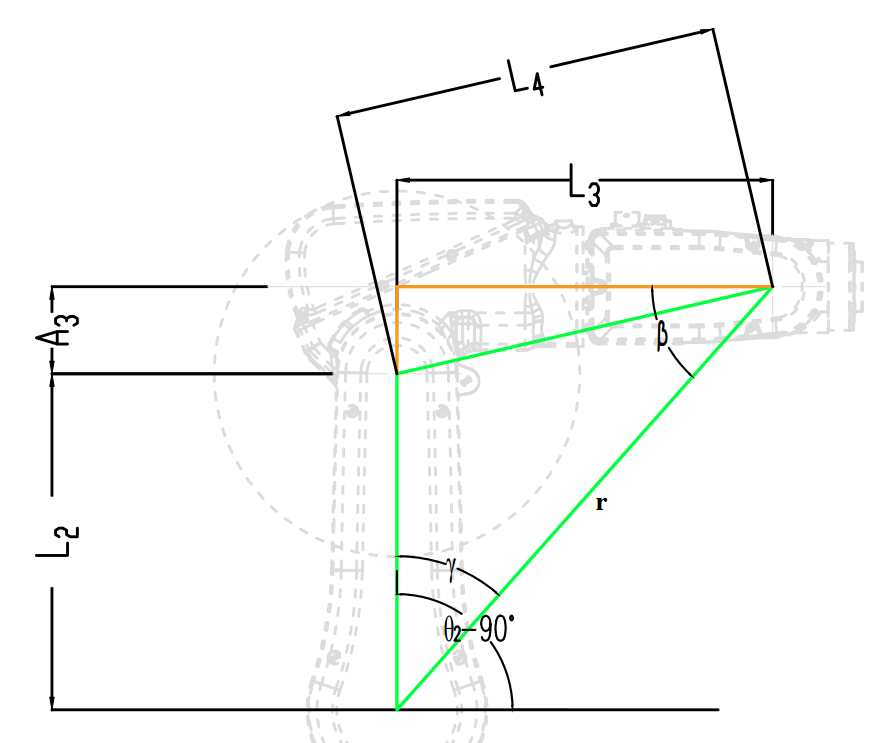
\includegraphics[width=0.75\textwidth]{Immagini/Theta_2_2}
	\caption{Triangoli di supporto per il calcolo del angolo $\theta_2$} 
	\label{fig:CalcoloTheta2}
\end{figure}

La lunghezza di $r$ dipende però ovviamente anche da altri angoli (quali $\theta_3$ per esempio): per procedere con il suo calcolo andiamo a ricavare le coordinate del polso (figura~\vref{fig:Coord_Polso}) espresse però nel sistema di riferimento 1 la cui origine si trova nel vertice dove è presente l'angolo $\theta_2-\ang{90}$, cioè dove si "ancora" il primo braccio del manipolatore. 

Quest'origine la possiamo definire andando a trovare la matrice di Denavit-Hartenberg relativa al sistema di riferimento 1 e poi, con una semplice moltiplicazione matriciale, siamo in grado di ottenere le coordinate del polso rispetto al punto prima specificato. 
\newpage
Conoscendo queste coordinate risulta facile calcolare sia il valore dell'angolo $\beta$ sia dell'angolo $\gamma$ (sfruttando il teorema di Carnot). 

Lo script \emph{MATLAB} risultante dai ragionamenti effettuati è il seguente:


\begin{lstlisting}[style=Matlab-editor,caption=Calcolo del parametro di giunto $\theta_2$,captionpos=b,label={Code:theta2}, basicstyle=\footnotesize\ttfamily,frame=trBL]

	%Parametri di Denavit-Hartenberg
	L2=270; %a_2
	L3=302; %d_4
	A3=70; %a_3	
	
	%Calcolo della lunghezza L_4
	L4 = sqrt(A3^2 + L3^2);

	%Matrice di trasformazione omogenea del primo giunto: indica orientamento e posizione del primo sistema di  riferimento rispetto alla base
	T01=Calcolo_DH_Matrix(robot, q, 1);	
	
	%Esprimo le coordinate del centro del polso rispetto alla base, utilizzando il concetto espresso in figura 2.18
	p1 = inv(T01)[Pm; 1];
	
	%Calcolo la distanza r, che dipende quindi dalla posizione del centro del polso e non risulta essere costante
	r = sqrt(p1(1)^2 + p1(2)^2);
	
	%Calcolo gli angoli espressi in figura 2.20, utilizzando i concetti matematici precedentemente esposti
	beta = atan2(-p1(2), p1(1));
	gamma = real(acos((L2^2+r^2-L4^2)/(2*r*L2)));	
	
	%Ho due possibili soluzioni: gomito su e gomito giu'
	q2(1) = pi/2 - beta - gamma;
	q2(2) = pi/2 - beta + gamma;
\end{lstlisting}




Per il calcolo di $\theta_3$ i parametri geometrici, ovvero le lunghezza dei lati dei triangoli presi in considerazione, sono sempre quelli presentati nel codice~\vref{Code:theta2}, cambia solamente il calcolo dell'angolo, come è ovvio che sia, il quale può essere così sviluppato:

\begin{lstlisting}[style=Matlab-editor,caption=Calcolo del parametro di giunto $\theta_3$,captionpos=b,label={Code:theta3}, basicstyle=\footnotesize\ttfamily,frame=trBL]

	%Calcolo degli angoli caratterizzanti
	phi=acos((A3^2+L4^2-L3^2)/(2*A3*L4));
	eta = real(acos((L2^2 + L4^2 - r^2)/(2*L2*L4)));
	
	%Due possibili soluzioni: gomito su e gomito giu
	q3(1) = pi - phi- eta; 
	q3(2) = pi - phi + eta; 
\end{lstlisting}



\begin{figure}[h]
	\centering
	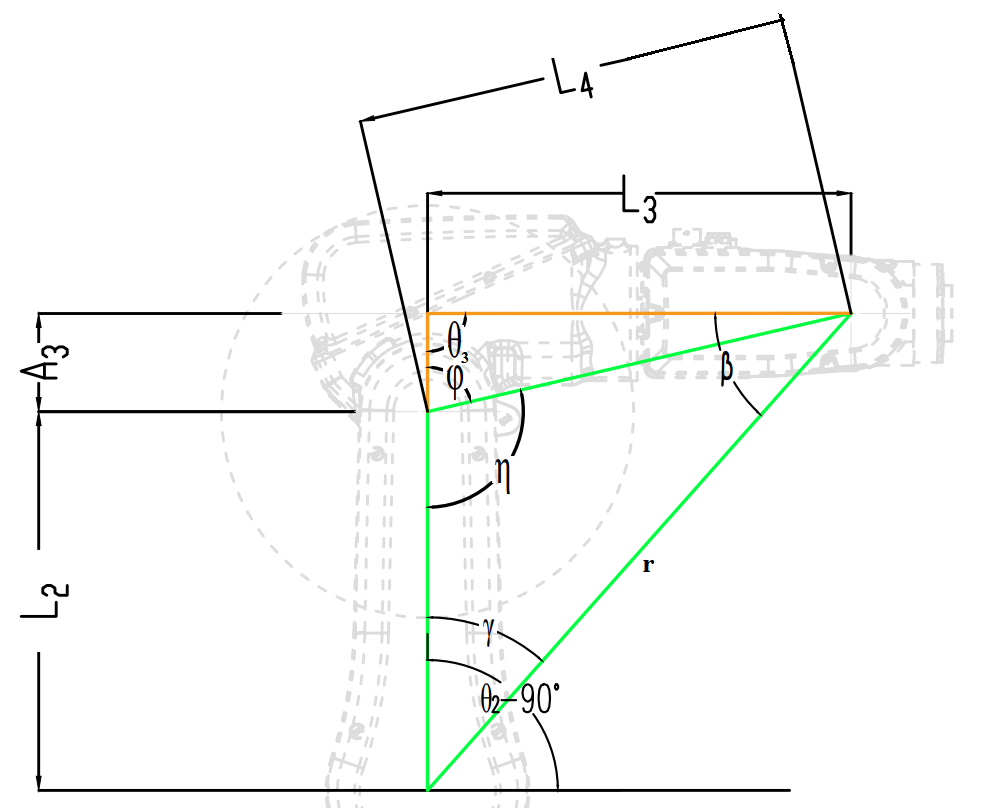
\includegraphics[width=0.75\textwidth]{Immagini/Theta_3}
	\caption{Triangoli di supporto per il calcolo del angolo $\theta_3$} 
	\label{fig:CalcoloTheta3}
\end{figure}



\subsection{Orientamento dell'end-effector: definizione variabili di giunto $\theta_4 - \theta_5 - \theta_6$}
Una volta calcolati i valori di $\theta_1 - \theta_2 - \theta_3$, la posizione del centro del polso risulta essere fissata: possiamo quindi calcolare la matrice di trasformazione omogenea che descrive la catena cinematica degli ultimi tre giunti.

\begin{lstlisting}[style=Matlab-editor,caption=Matrice  di trasformazione omogenea dei primi tre giunti,captionpos=b,label={Code:MatTrasf}, basicstyle=\footnotesize\ttfamily,frame=trBL]

	%Calcolo della posizione e dell'orientamento del terzo sistema di riferimento utilizzando gli angoli q (theta_1,theta_2,theta_3) prima calcolati
	T01=DH_Compute(robot, q, 1);
	T12=DH_Compute(robot, q, 2);
	T23=DH_Compute(robot, q, 3);
	T03=T01*T12*T23;
	
	%Vado ad estrarre le informazioni in merito alla rotazione del sistema di riferimento, come rappresentato in figura 2.10.
    x3=T03(1:3,1);
	y3=T03(1:3,2);
	z3=T03(1:3,3);
\end{lstlisting}
Questo listato fornisce la posizione del polso: quello che andiamo ora a fissare, definendo i tre angoli $\theta_4 - \theta_5 - \theta_6$ è l'orientamento del polso stesso, che può essere definito in termini di angoli di Eulero, ovvero di rollio-beccheggio-imbardata (\emph{Raw-Pitch-Yaw}). Come fatto precedentemente per individuare la posizione, anche qui abbiamo due vie di risoluzione: potremmo andare a risolvere il problema inverso tramite una via algebrica, la quale si basa sugli angoli individuati precedentemente ($\theta_1 - \theta_2 - \theta_3$) partendo dalla formula in figura~\vref{fig:AlgebricSolution}.
\begin{figure}
	\centering
	\caption{Step iniziale per il calcolo algebrico dell'orientamento del polso}
	\label{fig:AlgebricSolution}
	\begin{equation*}
		A_4A_5A_6 = (A_1A_2A_3)^{-1}		
		\begin{bmatrix}
		n_x & o_x & a_x & P_x\\
		n_y & o_y & a_y & P_y\\
		n_z & o_z & a_z & P_z\\
		0   & 0   & 0   & 1
		\end{bmatrix} 
	\end{equation*}
\end{figure}

Un altro possibile approccio, decisamente meno oneroso a livello computazionale, è rappresentato ancora una volta da quello geometrico: andando a lavorare sull'orientamento dei vari sistemi di riferimento rappresentati in figura~\vref{fig:CalcoloOrientamentoWrist} siamo in grado di recuperare i valori di $\theta_4 - \theta_5 -\theta_6$. 
\begin{figure}
	\centering
	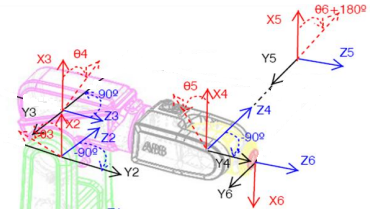
\includegraphics[width=0.75\textwidth]{Immagini/SistemiDiRiferimento_OrientamentoWrist}
	\caption{Sistemi di riferimento dei giunti utilizzati per trovare l'orientamento del polso} 
	\label{fig:CalcoloOrientamentoWrist}
\end{figure}

L'approccio che possiamo seguire per poter trovare l'angolo $\theta_4$ è quello di andare a studiare l'orientamento dell'asse $z_3$ e $z_6$, il quale è fornito in ingresso al problema cinematico inverso: valutando la posizione reciproca dei due assi sopracitati, possiamo andare a definire due casistiche di valori per $\theta_4$. In un caso esso è nullo, nell'altro può essere trovato andando sostanzialmente a costruire un triangolo rettangolo intorno a $\theta_4$, i cui lati possono essere considerati come gli assi $x_3$, $y_3$ e $z_3$.

Come si può notare nella figura~\vref{fig:CalcoloOrientamentoWrist}, $\theta_4$ è proprio l'angolo che si crea con $x_3$ e la trasposizione di $z_4$ sul giunto numero 3: operando un prodotto scalare, siamo in grado di trovare la proiezione di $z_4$ dapprima lungo $x_3$ e successivamente lungo $y_3$, grazie al significato geometrico proprio del prodotto scalare tra vettori.

Questi passaggi permettono di ottenere nient'altro che il valore del $cos$ e del $sen$ dell'angolo $\theta_4$, legati tra loro dalla funzione $atan$, come si può vedere nel codice~\vref{Code:theta4}.

\begin{lstlisting}[style=Matlab-editor,caption=Calcolo di $\theta_4$,captionpos=b,label={Code:theta4}, basicstyle=\footnotesize\ttfamily,frame=trBL]
	%Vado a calcolare la matrice di trasformazione omogenea del terzo giunto sfruttando le proprieta' delle matrici di trasformazione
	T01=DH_Compute(robot, q, 1);
	T12=DH_Compute(robot, q, 2);
	T23=DH_Compute(robot, q, 3);
	T03=T01*T12*T23;
	
	%Orientamento dei tre assi del sistema di riferimento del terzo giunto
	x3=T03(1:3,1);
	y3=T03(1:3,2);
	z3=T03(1:3,3);

	%Asse z_6 che corrisponde al vettore a nella matrice di trasformazione in input al problema cinematico inverso
	a=T(1:3,3);
	
	%Prodotto vettoriale: il risultato e' un vettore ortogonale al piano individuato da z_3 e z_6
	z4=cross(z3, a);   
	
	%Il modulo rappresenta l'area compresa tra i due assi: se e' circa nulla, vuol dire che i due assi sono paralleli, per le proprieta' del prodotto vettoriale
	if norm(z4) <= 0.000001
		q(4)=0;
	else
		%Vado a compormi un triangolo rettangolo, in base a quello che e' l'orientamento della sesta terna
		cq4=wrist*dot(z4, -y3);
		sq4=wrist*dot(z4, x3);
		q(4)=atan2(	sq4, cq4);
	end
\end{lstlisting}
\newpage
Anche per il calcolo di $\theta_5$ possiamo andare ad operare lo stesso ragionamento fatto per trovare $\theta_4$: in questo caso troveremo la proiezione dell'asse $z_5$, il quale fa riferimento al giunto 5 in esame, sugli assi del giunto precedente, ovvero su  $x_4$ e $y_4$.
\begin{lstlisting}[style=Matlab-editor,caption=Calcolo di $\theta_5$,captionpos=b,label={Code:theta5}, basicstyle=\footnotesize\ttfamily,frame=trBL]
	%Progressiva ricostruzione dell'orientamento e posizione della catena cinematica del manipolatore
	T34=DH_Compute(robot, q, 4);
	T04=T03*T34;
	x4=T04(1:3, 1);
	y4=T04(1:3, 2);
	
	%L'asse z_5 ha la stessa direzione di z_6
	z5=T(1:3, 3); 
	
	%Vado a lavorare sul triangolo rettangolo formato dagli assi	
	cq5=dot(z5, y4);
	sq5=dot(z5, -x4);
	q(5)=atan2(sq5, cq5);
\end{lstlisting}
Ripetiamo infine lo stesso concetto geometrico presentato per il calcolo di $\theta_4$ e $\theta_5$, anche per andare a trovare il valore di $\theta_6$.
\begin{lstlisting}[style=Matlab-editor,caption=Calcolo di $\theta_6$,captionpos=b,label={Code:theta6}, basicstyle=\footnotesize\ttfamily,frame=trBL]
	x6=T(1:3, 1);
	
	T45=DH_Compute(robot, q, 5);
	T05=T04*T45;
	x5=T05(1:3, 1);
	y5=T05(1:3, 2);
	
	cq6=dot(x6, -x5);
	sq6=dot(x6, -y5);
	q(6)=atan2(sq6, cq6);

\end{lstlisting}

\subsubsection{Quaternioni}
Nello studio della cinematica inversa si è analizzato come le variabili note a priori, per poter giungere alla soluzione del problema stesso, sono la posizione e l'orientamento dell'end-effector rispetto alla base del manipolatore stesso. 

Come visto nel paragrafo~\vref{subsub:Rot_elementari} si è in grado di esprimere la rotazione di una terna mobile rispetto ad una fissa traimite una matrice detta \emph{matrice di rotazione}: un modo però più conciso per poter esprimere l'informazione in merito alla rotazione è rappresentato dall'utilizzo dei quaternioni. 
Essi rappresentano delle entità in forma complessa che, data una matrice di rotazione in questa forma
\begin{equation}
	\centering
	\begin{bmatrix}
		x_1&y_1&z_1\\
		x_2&y_2&z_2\\	
		x_3&y_3&z_3
	\end{bmatrix}
\end{equation}
possono essere ottenuti come:
\begin{table}[h]
	\label{tab:Quaternion}
	\centering
	\begin{tabular}{cc}
			\midrule
			$q_1=\frac{\sqrt{x_1+y_2+z_3+1}}{2}$ & \\ 
			$q_2=\frac{\sqrt{x_1-y_2-z_3+1}}{2}$ & $sign q_2 = sign(y_3-z_2)$ \\
			$q_3=\frac{\sqrt{y_2-x_1-z_3+1}}{2}$ & $sign q_3 = sign(z_1-x_3)$ \\
			$q_4=\frac{\sqrt{z_3-x_1-Y_2+1}}{2}$ & $sign q_4 = sign(x_2-y_1)$ \\
			\bottomrule  
	\end{tabular}
\end{table}

\subsubsection{La funzione atan2}
\label{subsub:Function_atan2}
Sempre nella risoluzione della cinematica inversa, per andare a calcolare i 6 parametri di giunto, si vanno ad utilizzare concetti geometrici-matematici, richiamando soprattutto la geometria riguardante i triangoli rettangoli. 
Nello specifico, è importante saper gestire quello che è il corretto segno da assegnare agli angoli calcolati, e questo viene ad essere fatto tramite la funzione $\atantwo$ la quale segue il comportamento presentato in figura~\vref{fig:atan2}.

\begin{figure}[h]
	\centering
	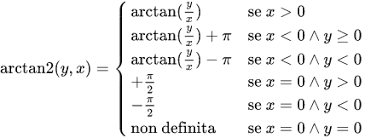
\includegraphics[width=0.65\textwidth]{Immagini/atan2}
	\caption{Caratteristiche della funzione $\atantwo$}
	%[Immagine presa dal sito https://it.wikipedia.org/wiki/Arcotangente2 in data 18/03/18]
	\label{fig:atan2}
\end{figure}
%======================================================================
%=====================================================================
	\chapter{Il controllore IRC5 Compact}
	\label{chapter:IRC5}
	
	%======================= DOCUMENTO ==================================================
Il manipolatore IRB 120 per poter essere gestito e per poter funzionare necessita di ricevere dall'esterno sia dei segnali di controllo che di alimentazione: di questo compito se ne occupa il controller IRC 5 Compact \emph{(Industrial Robot Controller)} (figura~\vref{fig:IRC5}), un'unità di controllo compatta che ha in sé tutti i benefici del IRC5, tra cui la precisione dell’analisi del movimento e l’utilizzo del
linguaggio di programmazione \textsc{rapid}, oltre a dimensioni nettamente ridotte.
\begin{figure}
	\centering
	\includegraphics[width=0.45\textwidth]{Immagini/IRC5}
	\caption{IRC5 Compact controller}
	\label{fig:IRC5}
\end{figure}

La parte di controllo della movimentazione, è individuata dalla presenza di un anello in retroazione sul sistema, in grado di valutare l'uscita e di andare a confrontarla con il valore di riferimento posto in ingresso. Questo feedback della traiettoria e della movimentazione non deve però essere esplicitamente sviluppato come un blocco a se stante, ma risulta già essere sviluppato all'interno del controllore stesso.
IRC5 Compact consente infatti ai robot di eseguire le proprie attività ad altissima efficienza, grazie ad una modellazione dinamica avanzata, permettendo di ottimizzare automaticamente le prestazioni riducendo i tempi di ciclo ($QuickMove^{TM}$) e garantendo che il percorso seguito dal robot sia lo stesso di quello programmato, indipendentemente dalla velocità di movimento ($TrueMove^{TM}$).

La tecnologia di IRC5 di ABB consente di prevedere il movimento del robot, garantendo prestazioni elevate, senza necessità di messa a punto da parte del programmatore, ovvero senza la necessità di dover andare a gestire il controllo sulla posizione.

\emph{Tu programmi, e lui esegue alla perfezione}.

Nella nostra applicazione, come in tutte le applicazioni che vanno a fare uso dei manipolatori industriali ABB, la presenza dell'IRC5 è inoltre fondamentale perchè permette di offrire una via per interfacciarsi e per gestire la movimentazione del braccio: questo è possibile grazie al fatto che esso supporta tutti i bus di campo attualmente in commercio in maniera tale che il robot possa integrarsi in ogni tipo di rete. 



Tra le numerose funzioni di networking ricordiamo il socket messaging (scambio di messaggi TCP/IP) e la possibilità di interfacciarsi con diversi sensori e accessi remoti: questo argomento è approfondito nella sottosezione~\vref{subsec:InterfaceIRC5}.

A livello "pratico", il controllore presenta delle interfacce destinate a gestire la parte di alimentazione e/o la parte di controllo del movimento del manipolatore: andiamo ora ad analizzare velocemente quelli che sono i principali collegamenti che il controllore offre.
\section{Pannello di controllo}
Il controller IRC5 presenta a bordo, oltre ad una serie di collegamenti, che gli permette di interfacciarsi al mondo esterno, anche una serie di pulsanti/interruttori situati sul pannello anteriore dell’IRC5 Compact.

\subsection{Pulsanti e interruttori}
La figura~\vref{fig:FrontPanelIRC5_1} mostra i pulsanti e gli interruttori situati sul pannello anteriore del controller IRC5 Compact.
\begin{figure}[h]
	\centering
	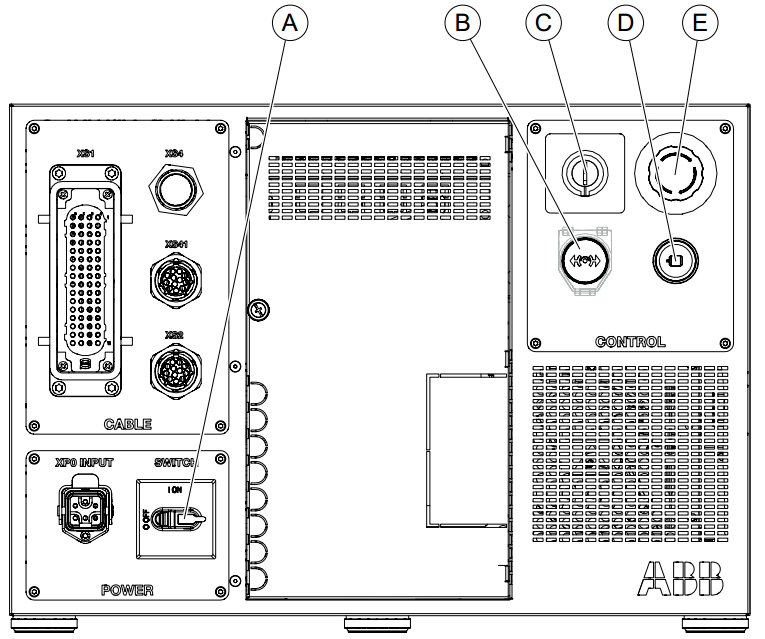
\includegraphics[width=0.5\textwidth]{Immagini/Pulsanti_Interruttori_IRC5}
	\caption{Pulsanti e interruttori presenti sul pannello anteriore del controller IRC5}
	\label{fig:FrontPanelIRC5_1}
\end{figure}
Le loro funzioni sono:
\begin{description}
	\item[A:] Interruttore principale di alimentazione
	\item[B:] Pulsante di rilascio dei freni che permette di modificare manualmente la posizione degli assi del manipolatore.
	\item[C:] Interruttore di scelta modalità di funzionamento del sistema robotico, la quale può essere: 
	\begin{itemize}
		\item \emph{Automatica}: definibile come “modalità di produzione” in cui il manipolatore si muove secondo quelle che sono le istruzioni RAPID (capitolo~\vref{text:RAPID}) che sono caricate a bordo del controllore. In questa modalità di funzionamento la velocità non risulta essere limitata, ma bensì dipende da quelle che sono le informazioni di velocità inserite all’interno della codifica delle istruzioni di movimento.
		\item \emph{Manuale}: in questa modalità il controllo avviene manualmente tramite il jog sulla flex pendant (figura ~\vref{text:FlexPendant}); la velocità di movimento risulta invece essere limitata a 250 mm/s.
	\end{itemize}
	\item[D:] Motori inseriti
	\item[E:] Arresto di emergenza: la pressione di questo tasto si rende necessaria nel momento in cui si attiva la modalità di funzionamento automatica. In particolar modo essa permette di attivare i motori che inizialmente risultano essere in blocco per motivi di sicurezza.
\end{description}
\subsection{Interfacce di collegamento}
\label{subsec:InterfaceIRC5}
Si analizzeranno, in prima battuta, le interfacce che permettono al controllore IRC5 di collegarsi al manipolatore IRB 120, fornendogli tutti i segnali necessari. In seconda battuta andremo ad  rapidamente i collegamenti che il controllore stesso presenta verso il "mondo esterno".
\newpage
Partiamo analizzando i collegamenti interni tra manipolatore e controller in figura~\vref{fig:FrontPanelIRC5_2}:
\begin{figure}[h]
	\centering
	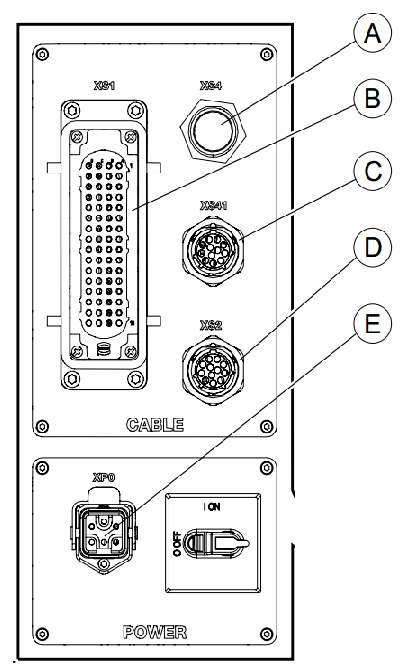
\includegraphics[width=0.3\textwidth]{Immagini/Connettori_IRC5}
	\caption{Connettori presenti sul pannello anteriore del controller IRC5}
	\label{fig:FrontPanelIRC5_2}
\end{figure}
\begin{description}
	\item[A:] Connessione alla FlexPendant
	\item[B:] Collegamento dell'alimentazione al robot
	\item[C:] Collegamento degli assi aggiuntivi
	\item[D:] Collegamento del robot
	\item[E:] Collegamento dell'alimentazione di rete
\end{description}
Il pannello di controllo dell’IRC5, oltre ai collegamenti esposti in precedenza, presenta altre porte di comunicazione, che permettono al controller di entrare in relazione con un PC/Sistema esterno.

In quello che è definito come il gruppo "computer" troviamo diversi collegamenti come si vede in figura~\vref{fig:ComputerGroup_IRC5}.
\begin{figure}
	\centering
	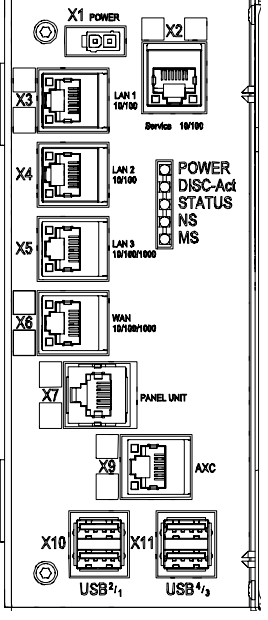
\includegraphics[width=0.30\textwidth]{Immagini/ConnettoriSulComputer}
	\caption{Porte di comunicazione IRC5}
	\label{fig:ComputerGroup_IRC5}
\end{figure}
I due collegamenti principali sono:
\begin{description}
	\item[Porta di servizio \textsl{X2}:]\label{item:Porta_servizio} questa porta è destinata ai tecnici di servizio e ai programmatori che si collegano direttamente al controller con un PC.
	La porta di servizio è configurata con un indirizzo IP fisso, che è identico per tutti i controller e non può essere modificato, ed è dotata di un server DHCP che assegna automaticamente un indirizzo IP al PC collegato: quindi, nel momento in cui si va a gestire la movimentazione del manipolatore tramite RobotStudio (capitolo~\vref{text:RAPID}), il PC deve essere connesso al controller tramite questa porta.
	Durante il collegamento il PC deve essere impostato su “Ottieni automaticamente un indirizzo IP” come descritto in Service PC information nel Boot Application della Flex Pendant (capitolo~\vref{chapter:FlexPendant}).
	
	\item[Porta di rete della fabbrica \textsl{X6}:] la porta di rete di fabbrica (WAN) è una porta pubblica destinata al collegamento del controller a una rete interna: per completezza si riporta in figura~\vref{fig:ComputerGroup_IRC5} una panoramica dei collegamenti possibili via Ethernet/USB. 
	Le impostazioni di rete possono essere configurate con qualsiasi indirizzo IP fornito, in genere, dall'amministratore della rete: per il PC dipendono dalla configurazione della rete medesima da parte dell’amministratore di rete.
	Questo ci permette di affermare che, un secondo modo per comunicare con il controllore, può essere tramite una rete (cablata o meno) alla quale risulta essere connesso il controllore stesso.
	Per la porta WAN non si possono utilizzare i seguenti indirizzi IP, in quanto già assegnati ad altre funzioni sul controller IRC5:
	\begin{itemize}
		\item 192.168.125.0 - 255
		\item 192.168.126.0 - 255
		\item 192.168.127.0 - 255
		\item 192.168.128.0 - 255
		\item 192.168.129.0 - 255
		\item 192.168.130.0 - 255
	\end{itemize}
	La porta WAN non può trovarsi su una subnet con uno degli indirizzi IP riservati sopra riportati. Se occorre utilizzare una subnet mask nell'intervallo B della classe di indirizzi, specificare un indirizzo privato di classe B per evitare conflitti.
\end{description}
\subsection{Morsettiera di suppporto}
Sul pannello di controllo dell'IRC5 Compact è inoltre presente una morsettiera che permette di effettuare collegamenti esterni (a livello \emph{"elettrico"}). Vediamo quelli che sono i principali collegamenti e le loro funzionalità.
\begin{description}
	\item[XS7-XS8-XS9] Questi connettori sono collegati internamente alla scheda di sicurezza e contengono i seguenti segnali:
	\begin{itemize}
		\item Arresto automatico
		\item Arresto generale
		\item Arresto di emergenza esterno
		\item Alimentazione esterna
	\end{itemize}
	\item[XS12\dots XS15] Questi connettori sono collegati internamente all'unità I/O: essi contengono 16 segnali di ingresso digitali, 16 segnali di uscita digitali,
	24 V e 0 V per le uscite e 0 V per gli ingressi. 24 V e 0 V devono essere di	alimentazione esterna.
	\item[XS16] Questo connettore è collegato internamente all'unità I/O e all'unità di
	distribuzione dell'alimentazione a 24 V con un assorbimento di corrente non superiore a 6A.
\end{description}
%====================================================================================
	\part{Il controllo del sistema}
	\label{part:Il_controllo}
	\chapter{Movimentazione manuale}
	%=============================================================
Una prima via per controllare il sistema, è rappresentata dalla modalità manuale:
essa permette di gestire direttamente, in \emph{tempo reale}, la posizioni di ognuno dei 6 giunti del manipolatore IRB 120, ad una velocità di movimento però limitata per questioni di sicurezza.

Ciò è possibile grazie alla \emph{Flex pendant} \label{text:FlexPendant}, in alcuni casi indicata anche come \emph{TPU} o Teach Pendant Unit, la quale è utilizzata per eseguire molte delle operazioni correlate al funzionamento di un sistema robotico: esecuzione dei programmi, movimentazione manuale del manipolatore, modifica di programmi a bordo del controllore ecc\dots\cite{ABB:Web_FlexPendant}.

Per capire quali sono gli utilizzi principali in cui la Flex Pendant ricopre un ruolo di primaria importanza, andiamo ad analizzare quelle che sono le principali parti \emph{fisiche} componenti l'unità stessa (figura~\vref{fig:FlexPendantParti}).
\begin{figure}[h]
	\centering
	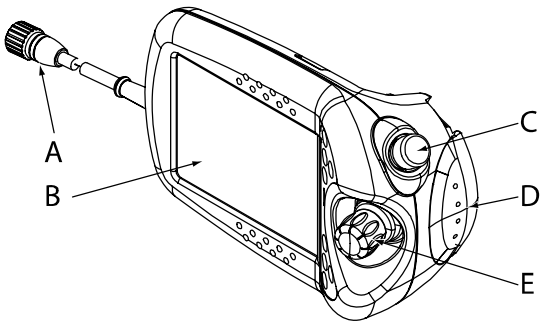
\includegraphics[width=0.5\textwidth]{Immagini/MainPart_TeachPendant}
	\caption{Componenti principali della Flex Pendant}{\cite{ABB:Web_FlexPendant}}
	\label{fig:FlexPendantParti}
\end{figure}

I componenti principali della Flex Pendant sono:
\begin{itemize}
	\item[A: ] Connettore
	\item[B: ] Touch screen
	\item[C: ] Pulsante di arresto di emergenza
	\item[D: ] Dispositivo di attivazione
	\item[E: ] Joystick
\end{itemize}

Si vede come, la Flex Pendant, sia decisamente adatta per la movimentazione manuale tramite il pratico joystick: esso permette di gestire contemporaneamente la movimentazione di tre assi per volta, unitamente ad un supporto visivo a schermo, che consente di configurare la movimentazione.
\begin{figure}[h]
	\centering
	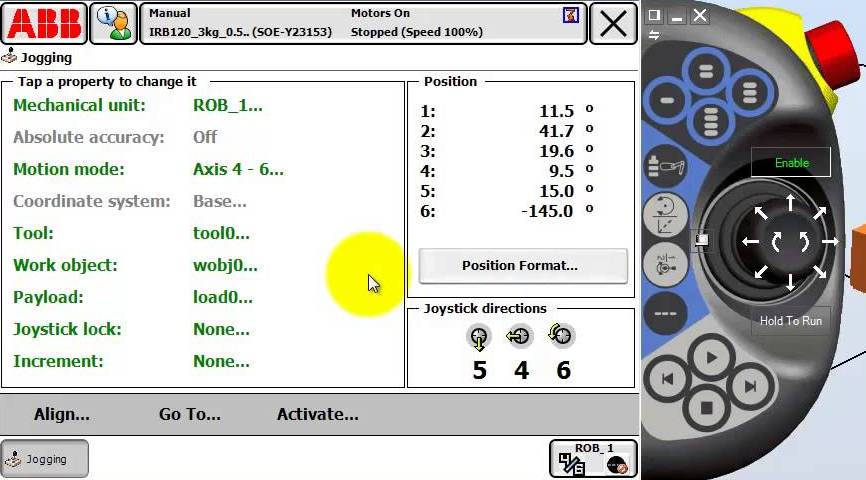
\includegraphics[width=0.5\textwidth]{Immagini/DisplayTPU_ManualJog}
	\caption{Schermata di controllo della movimentazione manuale tramite joystick}
	%[Immagine presa dal sito https://www.youtube.com/watch?v=cRQUxkt73is in data 25/02/18] 
	\label{fig:DisplayFlexPendant}
\end{figure}

Come si può vedere in figura~\vref{fig:DisplayFlexPendant}, la Flex Pendant permette di visualizzare, in tempo reale, la posizione dei 6 giunti, tramite una visualizzazione che può essere impostata in gradi oppure in radianti, fornendo anche la possibilità di gestire la movimentazione giunto per giunto oppure in maniera lineare o alternativamente secondo una tecnica circolare, a seconda delle esigenze specifiche. 

Si può inoltre andare a selezionare quale terna di giunti (1-2-3 o 4-5-6) sono oggetto di movimentazione tramite jog manuale, quale manipolatore, nei sistemi multimove, si vuole gestire potendo visualizzare allo stesso tempo anche i sistemi di coordinate alle quali il moto si riferisce.
Questa modalità di utilizzo rappresenta sicuramente un modo rapido e sicuro per gestire in maniera diretta la posizione del manipolatore: a livello di prestazioni e di funzionalità, come si può ben capire, è decisamente però una modalità molto limitante, al solo scopo dimostrativo e/o di setting-up.
%=============================================================
	\label{chapter:FlexPendant}
	\chapter{Movimentazione automatica}
	% !TeX spellcheck = <none>
%=================================================================================
\label{text:RobotStudio}Una soluzione decisamente più robusta, in grado di rendere la gestione della movimentazione più flessibile e precisa, è rappresentata dal controllo tramite l'ambiente di sviluppo ufficiale di ABB, il quale presenta nel software \emph{RobotStudio} l'elemento chiave.
\begin{figure}[h]
	\centering
	
\includegraphics[width=0.15\textwidth]{Immagini/Logo_RobotStudio}
	\caption{Logo RobotStudio}
	\label{fig:Logo_RobotStudio}
\end{figure}

RobotStudio è un applicazione distribuita uffucialmente da ABB il quale mette a disposizione tutti gli strumenti per aumentare la redditività del sistema robotizzato, consentendo di svolgere attività di formazione, programmazione e ottimizzazione senza interferire con la produzione: esso è basato su ABB Virtual Controller, una copia esatta del software che controlla il funzionamento dei robot in produzione. In questo modo si possono effettuare simulazioni 3D estremamente realistiche, utilizzando programmi e file di configurazione reali, identici a quelli usati sull'impianto produttivo reale.

Il punto centrale è proprio questo: RobotStudio mette a disposizione la possibilità di simulare, su PC, il funzionamento e il controllo del manipolatore, il quale, una volta terminato lo studio in un ambiente virtuale, potrà essere spostato sul controllore reale, che sarà poi in grado di determinare un controllo automatizzato del manipolatore stesso, permettendo di ottenere
\begin{itemize}
	\item Riduzione del rischio
	\item Avvio più veloce
	\item Meno tempo per le modifiche
	\item Aumento della produttivà
\end{itemize}
\emph{RobotStudio} mette a disposizione delle funzioni di utilizzo in una modalità d'uso detta \emph{offline}: questo significa che, quando RobotStudio funziona senza essere connesso ad un controller reale, esso permette di simulare, tramite un controller IRC5 virtuale su PC, il funzionamento del manipolatore. L'altra modalità di funzionamento è detta \emph{online}, e si attua nel momento in cui RobotStudio va ad agire direttamente su un controller reale.

Dall'istante in cui si va a lavorare in modalità online, è ovviamente necessario introdurre un collegamento tra il PC e il controllore: l'IRC5 Compact offre molte possibilità di collegamento; una prima opzione si presenta andando ad inserire il controller in una rete, per esempio in una rete interna di fabbrica, rendendo possibile la comunicazione di tutti i nodi della rete stessa con il controllore. 

Un modo decisamente più diretto per poter gestire la programmazione online, è rappresentato dal collegamento del controller al PC tramite la porta di servizio (~\vref{item:Porta_servizio}): con un semplice cavo Ethernet è possibile mettere in comunicazione il PC con il controller IRC5 Compact, per caricare il codice sorgente da eseguire a bordo del controller stesso, permettendo quindi un controllo del manipolatore in modalità online, la quale ci consentirà, come riportato nella sezione~\vref{subsec:ROS}, di aprire una comunicazione \emph{socket} per effettuare lo scambio di particolari tipologie di messaggi (definiti come \emph{package}).
\begin{figure}
	\centering
	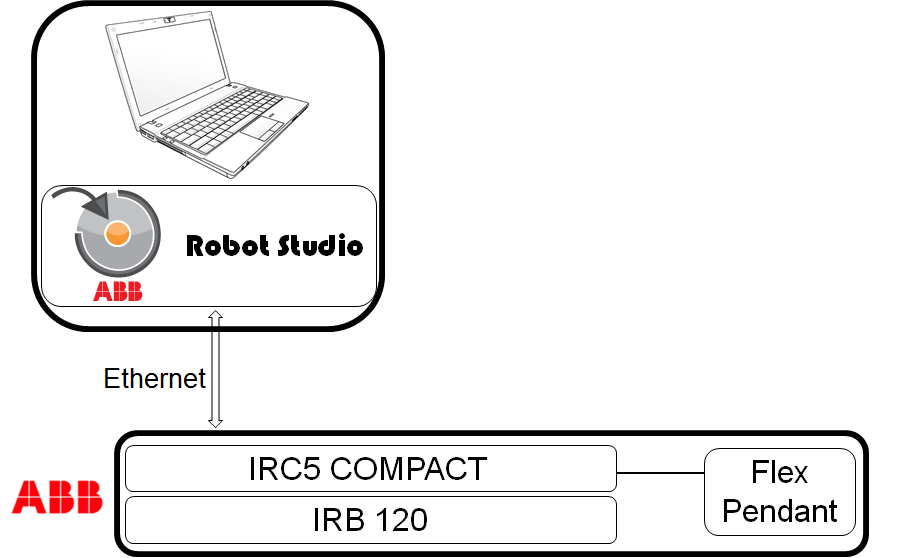
\includegraphics[width=0.75\textwidth]{Immagini/Automatic_SystemSchematic}
	\caption{Schema del funzionamento online del sistema di controllo automatico}
	\label{fig:SchematicAutomatic}
\end{figure}

\chapter{RobotStudio: programmazione statica}
\label{text:RAPID}
Come prima spiegato, \emph{RobotStudio} permette di effettuare una programmazione del movimento che può essere considerata statica: infatti, una volta parametrizzato e settato il codice da fornire al controller IRC5 Compact, non si ha la possiblità di interagire in "tempo reale" con il posizionamento del robot.

Ovviamente la caratteristica "saliente" di una gestione di questo tipo è il fatto che si può operare una pianificazione del movimento in ambito virtuale, sfruttando un controller simulato, il quale offre le stesse funzionalità del controllore fisico, ma solamente riportate su di una piattaforma virtuale.
\begin{figure}[h]
	\centering
	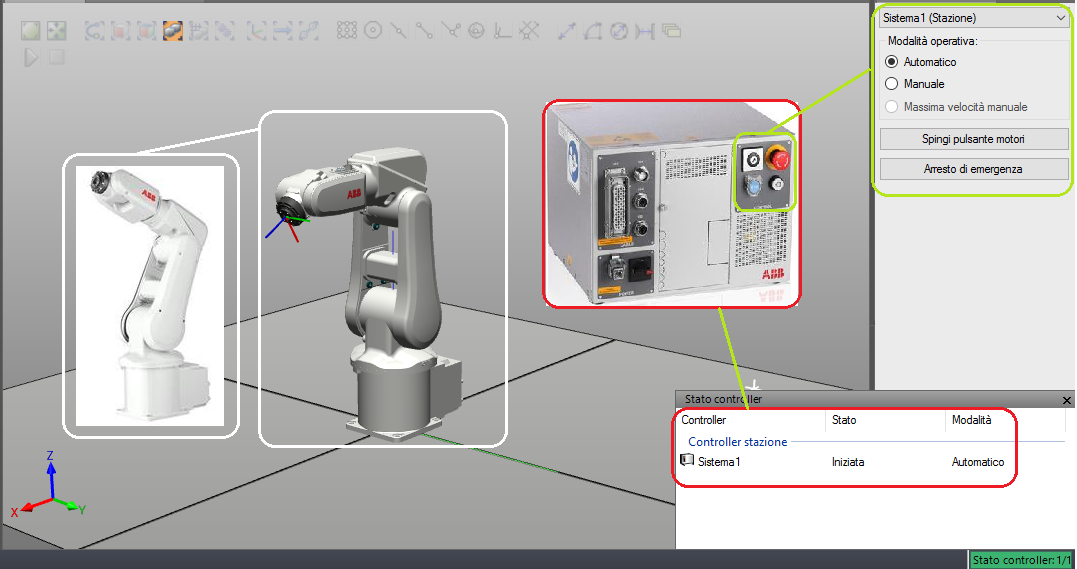
\includegraphics[width=0.85\textwidth]{Immagini/Virtual_System}
	\caption{Virtualizzazione del sistema fisico su piattaforma \emph{RobotStudio}}
	\label{fig:Virtual_sys}
\end{figure}

Nell'ambiente di sviluppo \emph{RobotStudio}, rappresentato nella figura~\vref{fig:Virtual_sys}, si ha un forte orientamento ad una programmazione \emph{statica}: il software mette infatti a disposizione la possibilità di andare a fissare dei sistemi di riferimento (\emph{target}) che, se inseriti all'interno di un percorso (\emph{path}), permettono di definire una movimentazione che il manipolatore poi potrà andare ad eseguire nella realtà, a patto che le posizioni definite dai target siano raggiungibili dal manipolatore stesso, rispettando i limiti e i vincoli geometrici.

La creazione di path è solamente una delle tante possibilità di virtualizzazione che \emph{RobotStudio} mette a disposizione: si possono andare a ricreare sistemi con geometrie molto più complesse come, per esempio, sistemi di saldatura (figura~\vref{fig:Complex_sys}) oppure di pick and place, permettendone così un'analisi del funzionamento e della gestione in maniera completamente svincolata dalla realtà.
Altre funzionalità implementate nell'ambiente di \emph{RobotStudio}, che permettono un controllo più capillare del manipolatore, sono:

\begin{itemize}
	\item Tabelle degli eventi: permettono di verificare la struttura del programma e la sua logica visualizzando gli stati degli I/O.
	\item Rilevamento delle collisioni: si tratta di uno strumento più orientato agli ambienti reali di operazione utilizzato per prevenire possibili collisioni del robot con l'ambiente esterno durante l'esecuzione del programma.
	\item Visual Basic for Applications (\emph{VBA}) per la creazione di interfacce di utilizzo 
\end{itemize}
Tutto questo è però possible, oltre a particolari motori grafici che permettono di modellizzare il sistema reale, anche grazie al linguaggio di programmazione \emph{RAPID}.
\begin{figure}
	\centering
	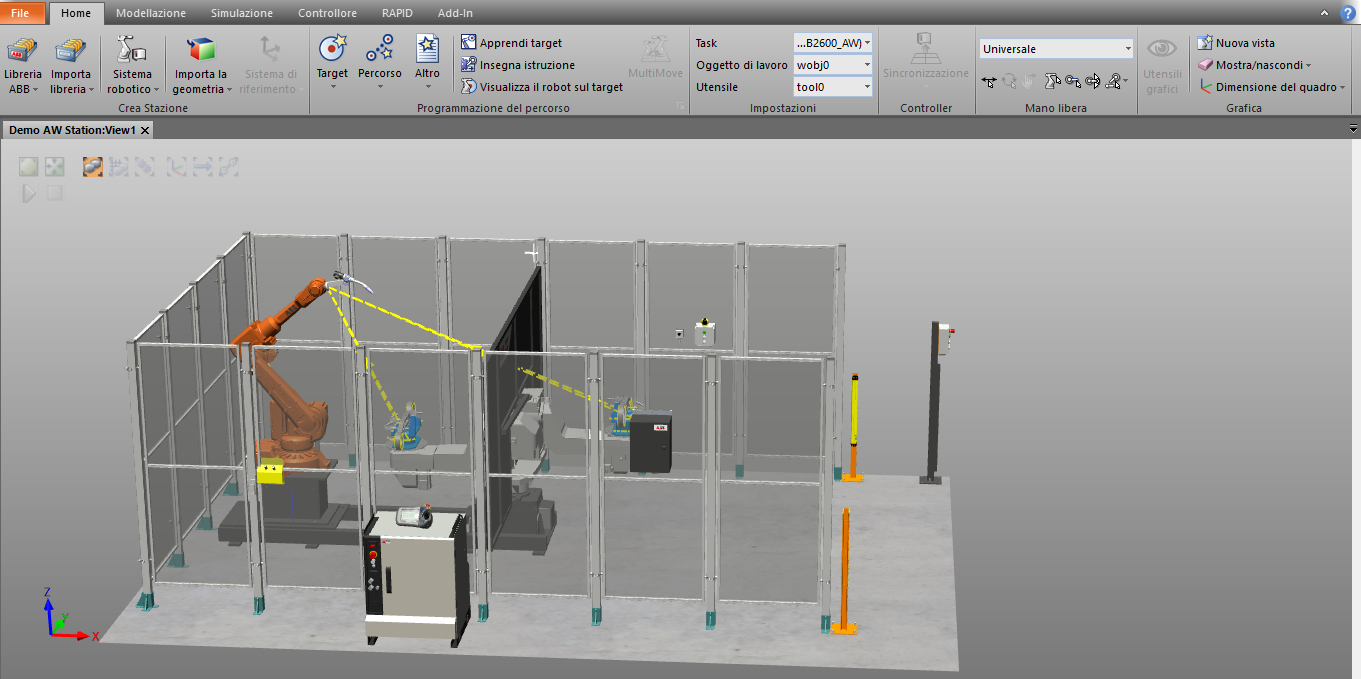
\includegraphics[width=0.8\textwidth]{Immagini/Complex_System}
	\caption{Esemplificazione del livello di complessità dei sistemi simulabili in \emph{RobotStudio}}
	\label{fig:Complex_sys}
\end{figure}

Il cuore della gestione sta quindi nella programmazione: si tratta di un linguaggio ad alto livello steso ad hoc da ABB nel 1994 per poter controllare e gestire la movimentazione dei propri manipolatori, tramite specifiche istruzioni che permettono di definire le modalità, le tempistiche e le velocità di movimento dei robot.
\begin{figure}[h]
	\centering
	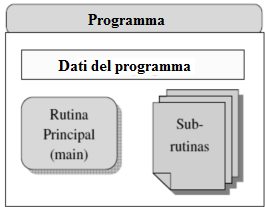
\includegraphics[width=0.45\textwidth]{Immagini/Struttura_RAPID}
	\caption{Schema base della struttura del programma \emph{RAPID}}
	\label{fig:Struttura_RAPID}
\end{figure}

Generalizzando, potremmo dedurre che il programma è una sequenza di istruzioni
che controlla il robot e che generalmente consiste di tre parti (figura~\vref{fig:Struttura_RAPID}): routine principale, subroutine e dati del programma.
\begin{itemize}
	\item Routine principale: routine dove si inizia l'esecuzione (main)
	\item Soubroutine: servono a dividere il programma in parti più piccole	per ottenere un programma modulare
	\item Dati del programma: definire posizioni, valori numerici, sistemi di
	coordinate, ecc. 
\end{itemize}

Quindi, oltre alle più comuni strutture e sintassi di programmazione, sono presenti particolari tipologie di istruzioni (istruzioni per spostare il robot oppure per impostare il valore di un determinato output), il cui comportamento è definito tramite argomenti che gli vengono passati in ingresso, e anche specifiche tipologie di dati, il cui ruolo è mirato ad una più facile gestione del movimento del robot, come si può facilmente notare nel listato~\vref{Code:ExampleRAPID}.

Tutte queste istruzioni che vanno a gestire la movimentazione e la traiettoria del manipolatore ABB possono essere raggruppate in uno o svariati moduli: ciascun modulo può contenere una o svariate procedure.
\label{Text:Mod_sys}
Si possono distinguere:
\begin{description}
	\item[Moduli di programma:] in essi viene memorizzato il codice RAPID che è individuato da un file che con estensione .mod (Module1.mod per esempio).
	Per il controller del robot non fa alcuna differenza se il programma è scritto in più moduli: il motivo di utilizzarne più di uno contemporaneamente in un programma è soltanto quello di rendere più facile la comprensione dello stesso, e agevolandone il riutilizzo da parte dei programmatori. Ovviamente, nonstante sia possibile avere più moduli installati sul controllore, è importante che solamente uno di essi contenga la procedura main, che verrà poi eseguita ripetutivamente dal controller.
	\label{text:SysModule}
	\item[Moduli di sistema:] questa particolare tipologia di moduli, salvati con estensione .sys, permettono di mantenere dati e procedure nel sistema, anche se il programma viene
	cambiato. Ad esempio, se una variabile persistente di tipo \emph{tooldata} viene dichiarata in un modulo di sistema, una calibrazione dell’utensile viene preservata, anche se venisse ad essere caricato un nuovo programma. 
	In questa tipologia di moduli non si ha però la possibilità di inserire delle soubrutine di \emph{main}: ciò significa che l'esecuzione del codice non potrà mai partire da questi moduli, ma dovrà iniziare sicuramente da moduli di programma, i quali poi potranno andare a richiamare le funzioni strutturate all'interno dei moduli di sistema.
\end{description}

\begin{lstlisting}[language=C++,style=Matlab-editor,caption=Esempio di programmazione \emph{RAPID},captionpos=b,label={Code:ExampleRAPID}, basicstyle=\scriptsize\ttfamily,frame=trBL]
MODULE Module1

	CONST robtarget HomePosition:=[[364.302,0,593.9999],[0.498,0,0.802,0],[0,0,0,0],[9E+09,9E+09,9E+09,9E+09,9E+09,9E+09]];
	% NB: La posizione e' definita rispetto al sistema di coordiante oggetto corrente
	CONST robtarget PosizioneIngresso_10:=[[515,325,75],[0,0.604,-0.5,0],[0,0,0,0],[9E+09,9E+09,9E+09,9E+09,9E+09,9E+09]];
	TASK PERS wobjdata Wobj_CellaPiante:=[FALSE,TRUE,"",[[200,200,0],[1,0,0,0]],[[0,0,0],[1,0,0,0]]]; 
	VAR robtarget TargetMobile;
	VAR num NumeroCicli := 0;
	VAR num m := 1;
	CONST robtarget PuntoIntermedio:=[[650,-215.8,150],[0.046,0.007,0.882,-0.002],[0,0,0,0],[9E+09,9E+09,9E+09,9E+09,9E+09,9E+09]];

	PROC main()
		IF (NumeroCicli = 0) THEN
			TPErase;
			%Per limitare le possibilita' di avere singolarita'
			SingArea\LockAxis4;
			MoveL HomePosition,v50,z5,tool0\WObj:=wobj0;
		ENDIF
		IF (NumeroCicli MOD m = 0 AND (NOT(NumeroCicli = 0))) THEN
			Y_Offset := 0;
			X_Offset := X_Offset -21;
		ENDIF
		TPWrite("Offset Y: "+ValToStr(Y_Offset));
		TPWrite("Offset X: "+ValToStr(X_Offset));
		TargetMobileEstrazione := Offs(PartenzaCellaEstrazione,X_Offset,Y_Offset,0);
		TargetMobile := Offs(PartenzaCella,X_Offset,Y_Offset,0);
		Y_Offset := Y_Offset - 22;
		NumeroCicli :=NumeroCicli+1;
	ENDPROC
ENDMODULE
\end{lstlisting}

Presentare però in questa sede il linguaggio \emph{RAPID}, con il giusto livello di approfondimento, sarebbe praticamente impossibile e, al contempo, fuoriluogo: per una maggiore trattazione si rimanda il lettore ai riferimenti \cite{ABB:Manul_RAPID} e \cite{ABB:CompleteManul_RAPID}.

\chapter{Programmazione dinamica: case study}
\label{subsec:ROS}
La pianificazione della traiettoria e la gestione della movimentazione in \emph{RobotStudio} è sicuramente molto "user-friendly": si ha la possibilità di generare automaticamente codice \emph{RAPID} a seconda di come viene configurato il sistema nella sezione di configurazione visuale, creando traiettorie ad hoc, con il minimo sforzo.

Il problema di un approccio di questo tipo è però che non si ha la possibilità di gestire in "tempo-reale" la movimentazione del robot: una volta caricato il listato \emph{RAPID} a bordo del controllore, esso lo eseguirà in maniera ciclica, fino a che non giungerà ad un punto di arresto inserito nel codice oppure fino a quando non verrà arrestato dell'esterno (tramite, per esempio, il fungo d'emergenza).

In progetti molto complessi vi è però spesso la necessità di creare traiettorie adattive, a seconda di quello che è lo stato dell'ambiente in cui il robot si trova a dover lavorare: è necessario quindi sapere gestire la movimentazione del manipolatore a seconda di quelle che sono le informazioni ricevute per esempio da fotocamere, sensori visuali etc. variando in maniera dinamica la posizione e l'orientamento del'end-effector, e quindi del robot stesso, in base al feedback ricevuto.
Nello studio delle diverse possibilità di controllo del manipolatore IRB 120 di ABB sono state prese in considerazioni molte alternative: si è pensato inzialmente di andare a fornire a \emph{RobotStudio} un file con estensione .txt contenente tutte le coordinate che il manipolatore avrebbe dovuto raggiungere. In questa pirma soluzione la parte dinamica sarebbe stata fornita da una scrittura continua del file .txt delle coordinate, in maniera tale che il codice statico struttrato in ambiente \emph{RAPID} potesse poi andare gestire in maniera iterativa la posizione del manipolatore.

Una seconda soluzione presa in considerazione, è stata quella di utilizzare un metodo di controllo basato sulla comunicazione tramite \emph{OPC Server}: OPC (OLE for Process Control) è uno standard di comunicazione nel campo di controllo e supervisione dei processi industriali, basato su una tecnologia Microsoft, che offre un'interfaccia comune per la comunicazione consentendo a singoli componenti software di interagire e condividere dati attraverso un'architettura client-server, il cui ipotetico schema, nel caso di implementazione, sarebbe potuto essere quello in figura~\vref{fig:OPC_Connection}.
\begin{figure}
	\centering
	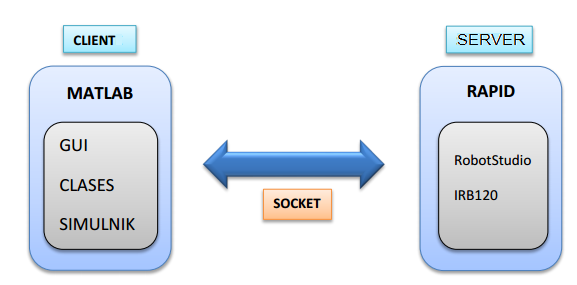
\includegraphics[width=0.75\textwidth]{Immagini/OPC_Configuration}
	\caption{Configurazione di una comunicazione OPC tra client e server}
	\label{fig:OPC_Connection}
\end{figure}

Questo tipo di soluzione è decisamente performante poichè permette di andare a lavorare in ambiente \emph{MATLAB}, tramite alcuni toolbox dedicati che consentono una gestione maggiormente ottimizzata della cinematica inversa, con la possibilità anche di andare a lavorare con sistemi costruiti tramite blocchi in ambiente Simulink.

La terza soluzione, presa poi effettivamente in considerazione, è stata quella di andare ad utilizzare ROS per gestire dinamicamente la traiettoria del manipolatore, a seconda dello stato dell'ambiente: quindi, per la disponibilità di informazioni reperibili sul web, unitamente ad un \emph{know-how} di partenza in ambiente di sviluppo Ubuntu, è stato scelto di andare a seguire e sviluppare un controllo basato su questa opzione.

\chapter{ROS: \emph{Robot Operating System}}
\begin{figure}[h]
	\centering
	
\includegraphics[width=0.3\textwidth]{Immagini/Logo_ROS}
	\caption{\emph{Robot Operating System}}
	\label{fig:LogoROS}
\end{figure}
Andiamo ora ad introdurre, all'interno di questo progetto, una piattaforma software chiamata \emph{Robot Operating System}, più comunemente detta ROS, la quale risulta essere frutto di un enorme sviluppo subito negli ultimi anni dalla comunità della robotica, il quale ha permesso la creazione di algoritmi e ambienti in grado di andare a gestire piattaforme robotiche con un sempre maggiore livello di autonomia e intelligenza.
\begin{figure}[h]
	\centering
	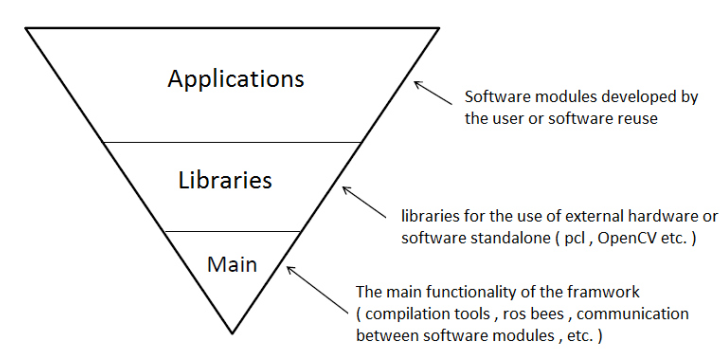
\includegraphics[width=0.75\textwidth]{Immagini/ROS_ComponentBased}
	\caption{Struttura a componenti di ROS}
	\label{fig:ROS-ComponentBased}
\end{figure}

ROS, come si può vedere \cite{online:ROS-Page}, è definibile come:
\begin{center}
	\emph{ROS è un sistema operativo open-source, con una struttura basata su componenti, che fornisce librerie e tools per aiutare gli sviluppatori a creare robot applications. Esso fornisce astrazione dell'hardware, driver dei dispositivi, librerie, strumenti di visualizzazione, comunicazione a scambio di messaggi tra processi (message passing), gestione dei pacchetti e molto altro}.\\	
\end{center}
Prima di entrare nello studio dell'architettura della nostra applicazione, risulta essere utilie andare ad introdurre quelli che sono i componenti principali: ROS, essendo infatti un sistema operativo, crea una rete (figura~\vref{fig:ROS-Network}) dove tutti i processi sono connessi tra di loro. 
\begin{figure}[h]
	\centering
	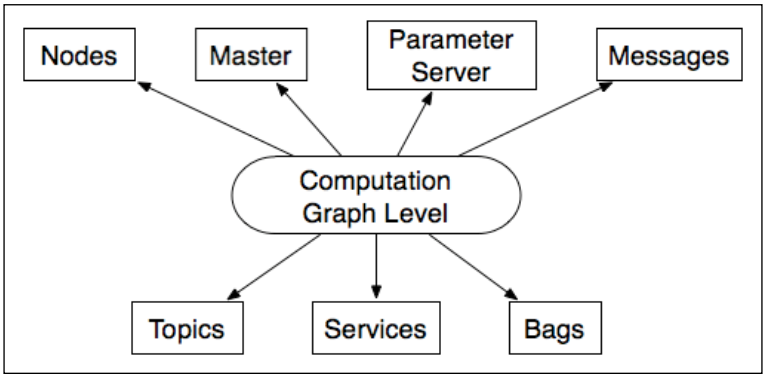
\includegraphics[width=0.75\textwidth]{Immagini/ROS_Network}
	\caption{Concetti fondametali su cui si basa una "network" ROS}
	\label{fig:ROS-Network}
\end{figure}

Nello specifico, all'interno di questa rete, possiamo andare ad individuare diversi elementi caratterizzanti, quali:
\begin{description}
	\item[\underline{Nodes}:] un \emph{nodo} è un processo che esegue delle operazioni di calcolo, fornendo così un modo per poter andare a dividere le funzionalità del sistema in più blocchi, semplificandone di molto il funzionamento e l'utilizzo.
	Le operazioni a cui si fa riferimento sono sostanzialmente implementate tramite l'utilizzo di diverse librerie (ROS client library) come roscpp, che permette di produrre nodi scritti in C++, oppuree rospy, per l'ambiente Python.
	Ogni nodo può andare a comunicare con altri nodi attrraverso \emph{topics}, RPC services oppure tramite \emph{Parameter server}. 
	
	Per comprendere meglio il concetto di nodo, è bene evidenziare come, in un sistema di controllo per sistemi robotici, sono compresi solitamente più nodi, uno per esempio va a controllare gli azionamenti delle ruote, uno ne computa la posizione e un'altro ancora ne calcola il percorso (\emph{path planning}) etc.
	
	Ad ogni singolo nodo è associato un nome univoco all'interno del sistema, in maniera tale che la comunicazione tra di essi possa avvenire senza ambiguità.
	In particolar modo, l'architettura "a nodi" che caratterizza il sistema ROS si basa sul concetto di.
	\begin{itemize}
		\item[Roscore:] il nodo roscore, considerabile come il nodo master, è l'elemento fondamentale che si occupa di andare a coordinare la connessione tra i nodi che sono legati a roscore stesso gestendone la comunicazione.
		\item[Rosnode:] esso rappresenta la tipologia di nodi sviluppati dall'utente, tramite la stesura di codice (solitamente C++ oppure Python).
	\end{itemize}
	\begin{figure}[h]
		\centering
		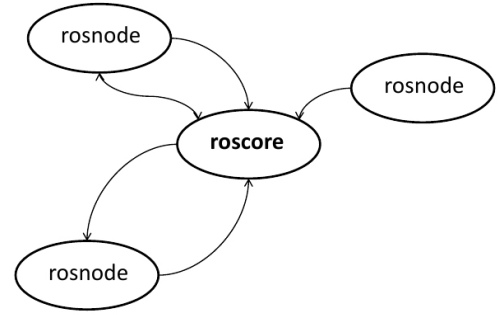
\includegraphics[width=0.75\textwidth]{Immagini/Ros_Core_Node}
		\caption{Elementi principali dell'architettura ROS}
		\label{fig:RosCoreNode}
	\end{figure}

	\item[\underline{Topics}:] essi non sono altro che "bus" attraverso i quali i nodi vanno a scambiarsi messaggi, rendendo possibile una programmazione multi-thread, ignorando i problemi relativi alla sincronizzazione tra processi. Nello specifico, tramite l'utilizzo di topics, si va a creare una semantica "anonima" di comunicazione, definita \emph{publish-subscribers}\label{text:pubsub}, che permette di disaccoppiare, come detto in precedenza, le parti di produzione delle informazione da quelle che le informazioni invece vanno a consumarle.
	
	In questo protocollo di comunicazione e scambio di messaggi, i nodi non sono a conoscenza del destinatario con cui stanno comunicando. Essi sono invece interessati al tipo di dati che si vanno a scambaire tramite un certo topic: infatti, ogni singolo topic, è fortemente tipizzato da ROS, il chè gli consente di avere più subscribers, ma un solo tipo di dato.
	\begin{figure}[h]
		\centering
		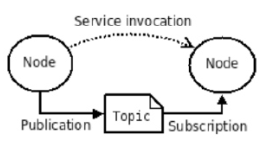
\includegraphics[width=0.70\textwidth]{Immagini/PubSub}
		\caption{Comunicazione basata sul protocollo \emph{publisher-subscribers}}
		\label{fig:PubSub}
	\end{figure}
	
	Questo significa che tramite un dato topic, i nodi che vi sono connessi (\emph{subscribers}), possono scambiarsi solamente una certa tipologia di messaggi: quindi è molto importante sottolineare il fatto che un nodo può diventare \emph{publisher} su un certo topic, solamente se il tipo di messaggio che vuole pubblicare coincide con quello "caratterizzante" il topic in questione e allo stesso tempo può sottoscrivere un topic solamente se la tipologia dei messaggi coincide con quella trattata.
	
	\item[\underline{Services}:] il modello publish/subscriber è sicuramente un paradigma di comunicazione molto flessibile, ma il suo trasporto unidirezionale \emph{molti a molti} non è appropriato per le interazioni di richiesta e risposta tipiche della comunicazione tra nodi. Questo concetto di richiesta/risposta è quindi realizzato tramite \emph{service}, come si vede nella figura \ref{fig:PubSub}, il quale è definito da una coppia di messaggi: uno per la richiesta e uno per la risposta.
	In sostanza un nodo ROS offre un servizio, sotto un certo nome, a tutti gli altri nodi del sistema, i quali possono richiedere il dato servizio iniviando il messaggio di richiesta, attendendone poi la risposta.
	\item[\underline{Messages}:] i nodi comunicano tra di loro pubblicando messaggi all'interno dei topics; nello specifico, questi messaggi sono rappresentati da una semplice struttura di dati, comprendente dei campi tipizzati. Come evidenziato nel punto precedente, i nodi possono anche scambiarsi un messaggio di richiesta e risposta come parte di una chiamata di servizio ROS i quali  sono definiti nei file srv. 
\end{description}
\begin{figure}[h]
	\centering
	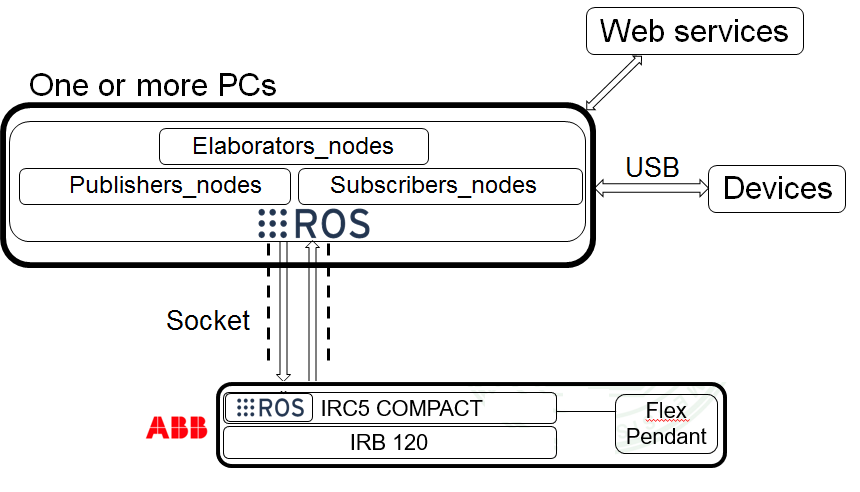
\includegraphics[width=0.75\textwidth]{Immagini/ROS_UniBG_Structure}
	\caption{Struttura architetturale di massima del sistema}
	\label{fig:ROS-UniBG}
\end{figure}
Gli elementi sicuramente caratterizzanti la comunicazione e lo scambio di informazioni all'interno di ROS sono sicuramente i nodi, i quali rappresentano programmi esecutivi che si scambiano dati attraverso topics: ogni singolo topic ha un proprio nome e può accettare solamente un tipo di messaggio.

In ROS sono inclusi molti tipi di messaggi, a seconda della tipologia di informazioni che si ha la necessità di trasmettere: un esempio di messaggio utilizzato molto spesso all'interno di questo progetto è "\emph{geometry\_msgs/Pose}", il quale ha una propria struttura interna composta da 7 variabili di tipo float, 3 delle quali definiscono la posizione e 4 invece rappresentano l'orientamento (espresso in quaternioni).

Per mandare messaggi è quindi necessario eseguire un'azione di \emph{publish} su uno specifico topic per quella data tipologia di messaggi; per riceverli è invece necessario fare un'azione di \emph{subscribe}, ovvero sottoscriversi ad un determinato topic.
\begin{lstlisting}[style=Matlab-editor,caption=Semplice esempio di comunicazione publish-subscribe,captionpos=b,label={Code:pubsub-example}, basicstyle=\scriptsize\ttfamily,frame=trBL]

	%Node 1:
	#include geometry\_msgs/Pose.h
	ros:: Publisher pub = n.advertise<geometry\_msgs::Pose>("object_position",10);
	pub.publish(send\_position);
	
	%Node 2:
	ros::Subscriber sub
	handle_function(geometry\_msgs/Pose received\_position)
	 {
	 	...
	 }
	 ros::Subscriber sub = n.subscribe("object\_position",10,handle_function);
\end{lstlisting}


\section{ROS industrial e IRB 120}
La struttura di ROS presentata in precedenza rappresenta un'architettura generica, la quale però non fornisce gli strumenti adatti per poter andare a gestire la traiettoria e la movimentazione dei manipolatori utilizzati in ambito industriale. Le potenzialità dell'ambiente ROS possono però essere estese anche all'ambito manifatturiero e produttivo, permettendo così di realizzare applicazioni robotiche di produzione che in precedenza erano tecnicamente irrealizzabili e proibitive.

Questo è possibile grazie a \emph{ROS-I} (ROS Industrial) il quale, tramite la presenza di molte repository open source disponibili online, fornisce interfacce per i più diffusi manipolatori industriali, end-effector, sensori e dispositivi connessi in rete, fornendo molti benefici, sostanzialmente dovuti alla forte struttura stratificata che \emph{ROS-I} fornisce (figura~\vref{fig:RosIStructure}).
\begin{itemize}
	\item Aumentare le potenzialità di ROS
	\item Applicare la strada a nuove applicazioni
	\item Rendere la programmazione dei robot più ad alto livello
	\item Ridurre i costi
	\item Essere totalmente open-source con una corposa communità di ricerca e sviluppo 
\end{itemize}

\begin{figure}[h]
	\centering
	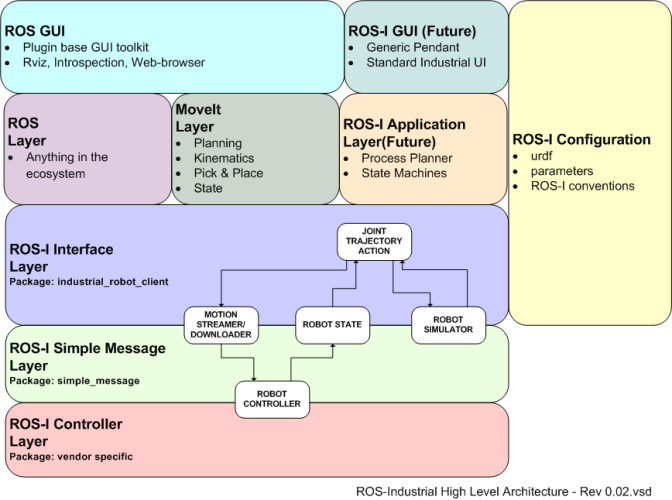
\includegraphics[width=0.75\textwidth]{Immagini/ROS_I_Structure}
	\caption{Architettura ad alto livello di ROS Industrial}
	\label{fig:RosIStructure}
\end{figure}

Volendo quindi andare a gestire la movimentazione di un manipolatore ABB, dovremo essere in grado di dare a \emph{ROS-I} le giuste informazioni in merito alla geometria del robot stesso unitamente alle caratteristiche intrinseche: questo è possibile grazie ai pacchetti software che ROS-Industrial mette a disposizione.
Tali pacchetti possono essere suddivisi in 
\begin{itemize}
	\item Pacchetti software generici, in grado di fornire delle implementazioni non specifiche
	\item Pacchetti software specifici, i quali forniscono supporto per il setup e la configurazione di molte piattaforme robotiche
\end{itemize}
Tra questi pacchetti specifici, troviamo anche quelli che permettono di andare ad eseguire un setup dell'ambiente ROS per quanto riguarda i manipolatori della linea di ABB.
Andiamo quindi ora ad analizzare nello specifico quella che è la struttura \emph{publish-subscriber} che il pacchetto ABB implementato in \emph{ROS-I} mette a disposizione.

\section{Comunicazione socket: concetti base}
Come già precedentemente presentato, il classico flusso di lavoro e di comunicazione tra il robot IRB 120 e il controller IRC5 Compact è schemtizzabile in alcuni semplici passi quali, andare a creare un programma in linguaggio RAPID, simularlo in RobotStudio e caricarlo poi a bordo del controller IRC5 per poterlo eseguirlo.
\begin{figure}[h]
	\centering
	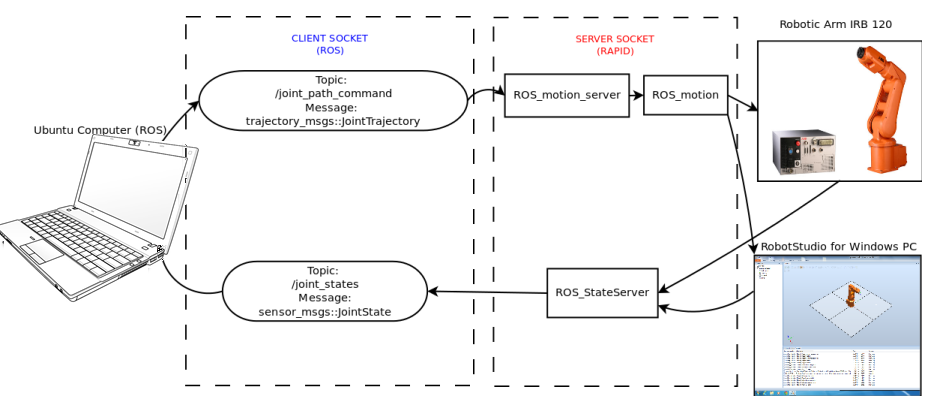
\includegraphics[width=0.75\textwidth]{Immagini/Socket_Comm}
	\caption{Schematizzazione della comunicazione socket tra client e server con relativo flusso di dati}
	\label{fig:SocketStructure}
\end{figure}
Il nostro obbiettivo è quello però di andare ad effettuare un controllo esterno, permettendo l'esecuzione di applicazioni più complesse, come quelle che includono sistemi sensoristici: questa esigenza può essere soddisfatta andando ad utilizzare un socket per permettere al client, ovvero ai nodi in ambiente ROS, di comunicare con il server, che nel nostro caso sarà rappresentato dal controller IRC5 Compact.

Un socket è oggetto software che permette l’invio e la ricezione di dati, tra host remoti (tramite una rete) o tra processi locali (Inter-Process Communication).
Più precisamente, il concetto di socket si basa sul modello Input/Output su file di Unix, quindi sulle operazioni di open, read, write e close; l’utilizzo, infatti, avviene secondo le stesse modalità, aggiungendo i parametri utili alla comunicazione, quali indirizzi, numeri di porta e protocolli.
\begin{figure}[h]
	\centering
	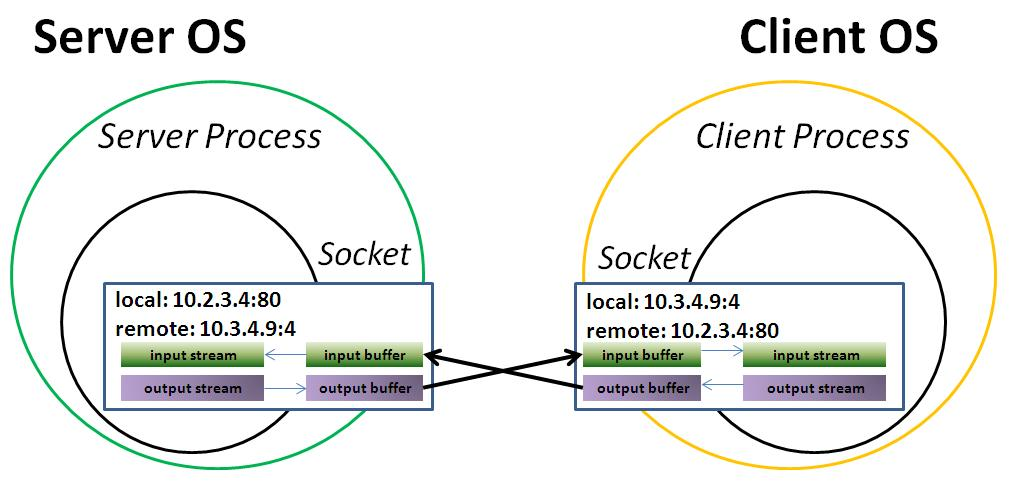
\includegraphics[width=0.75\textwidth]{Immagini/Basic_SocketConfig}
	\caption{Configurazione schematica della comunicazione socket}
	\label{fig:BasicSocketConfig}
\end{figure}

Con tale termine (che letteralmente vuol dire “presa”), in generale, si definisce una rappresentazione a livello software utilizzata per interfacciare due terminali (endpoint) in gioco in una connessione. In altre parole, potremmo considerare i socket come delle prese (una per ogni macchina) che siano interconnesse tra loro attraverso un ipotetico cavo in cui passi il flusso di dati che i computer si scambiano.

Un esempio che rende bene l’idea è quello di pensare ai socket come alle prese telefoniche presenti ai due capi opposti durante una conversazione al telefono. Le due persone che parlano al telefono, comunicano attraverso le rispettive prese. La conversazione, in tal caso, non finirà finché non verrà chiusa la cornetta e fino ad allora la linea resterà occupata.
Questa conversazione deve però essere univocamente individuata dato che, sui sistemi interlocutori, possono esserci molti processi: bisogna quindi avere un modo per indirizzare precisamente il processo con cui si sta dialogando, utilizzando le porte, ovvero numeri che identificano i processi in esecuzione.
Gli interlocutori, quindi, memorizzano indirizzo e porta della controparte, in un indirizzo socket, così formato:
\begin{itemize}
	\item  Indirizzo IP (32 bit)
	\item  Numero di porta (16 bit)
\end{itemize}
In base a come avviene la comunicazione, ovvero lo scambio di pacchetti, si possono avere diverse tipologie di comunicazione socket: in questa applicazione si va a sfruttare la solidità del protocollo TCP (come si può vedere nel listato~\vref{Code:SocketTCP} dove non è specificato l'argomento UDP),
\begin{lstlisting}[style=Matlab-editor,caption=Istruzione RAPID di creazione del socket,captionpos=b,label={Code:SocketTCP}, basicstyle=\tiny\ttfamily,frame=trBL]
IF (SocketGetStatus(server_socket) = SOCKET_CLOSED) SocketCreate server_socket;
\end{lstlisting}
 il quale garantisce una comunicazione affidabile, full-duplex, e con un flusso di byte di lunghezza variabile: essa prende il nome di \emph{Stream socket} e presenta sostanzialmente 4 fasi ben definite, che poi andremo anche a ritrovare nella parte di codice \emph{RAPID}:

\begin{description}
	\item[Creazione del socket:] client e server creano i loro rispettivi socket, e il server lo pone in ascolto su una porta.
	Dato che il server può creare più connessioni con client diversi (ma anche con lo stesso), ha bisogno di una coda per gestire le varie richieste.
	\item[Richiesta di connessione:] il client effettua una richiesta di connessione verso il server.
	Da notare che possiamo avere due numeri di porta diversi, perchè una potrebbe essere dedicata solo al traffico in uscita, l’altra solo in entrata; questo dipende dalla configurazione dell’host.
	In sostanza, non è detto che la porta locale del client coincida con quella remota del server: il server riceve la richiesta e, nel caso in cui sia accettata, viene creata una nuova connessione.
	\item[Comunicazione:] ora client e server comunicano attraverso un canale virtuale, tra il socket del primo, ed uno nuovo del server, creato appositamente per il flusso dei dati di questa connessione.
	È possibile, quindi, che ci siano molti client a comunicare con il server, ciascuno verso il data socket creato dal server per loro.
	\item[Chiusura della connessione:] essendo il TCP un protocollo orientato alla connessione, quando non si ha più la necessità di comunicare, il client lo comunica al server, che ne deistanzia il data socket.
	La connessione viene così chiusa.
\end{description}
\section{Messaggio custom scambiato tramite socket}
\label{text:MessaggeProtocol}
La comunicazione tra client e server, la cui struttura interna sarà spiegata nelle sezioni~\vref{sec:Client} e~\vref{sec:Server}, avviene tramite l'apertura di una connesione socket basata su un protocollo di trasporto di tipo TCP, il quale garantisce una comunicazione più sicura e controllata. Nello specifico client e server si scambiano messaggi che hanno una struttura predefinita, in maniera tale che entrambi siano in grado di interpretare i dati ricevuti/spediti.
Ovviamente questa struttura deve essere definita all'interno dei file di supporto presenti all'interno del \emph{catkin workspace} installato in ambiente Unix: il file che specifica la struttura del messaggio è il file \emph{simple\_message.h} che può essere trovato sotto il percorso \emph{ catkin\_ws\textbackslash src\textbackslash industrial\_core \textbackslash simple\_message\textbackslash include\textbackslash simple\_message.h}.

All'interno di questo file si può vedere come il messaggio sia strutturato in 3 macro-parti:
\begin{description}
	\item[Prefix:] non è considerato parte del messaggio e contiene la lunghezza, in bytes, dell'intero messaggio composto da Header+Body 
	\item[Header:] è formato sostanzialmente da 3 sotto campi i quali rappresentano dei parametri che consentono una corretta identificazione del tipo di messaggio (\emph{message type code}) che si sta mandando e dello stato della comunicazione. Questi campi sono:
	\begin{description}
		\item[MSG\_TYPE: ]permette di identificare il tipo di messaggio tramite dei valori standard e specifici a seconda del tipo di robot con cui si sta lavorando, tramite la dichiarazione di un'enumerazione, come si può vedere nel listato~\vref{Code:MSGTYPE_Param}, il quale è definito sempre all'interno del file \emph{simple\_message.h}.		
		\begin{lstlisting}[style=Matlab-editor,caption=Definizione dei parametri del campo MSG\_TYPE,captionpos=b,label={Code:MSGTYPE_Param}, basicstyle=\tiny\ttfamily,frame=trBL]
			namespace StandardMsgTypes
			{
				enum StandardMsgType
				{
					INVALID = 0,
					PING = 1,
					
					JOINT_POSITION = 10,
					JOINT = 10, 
					READ_INPUT = 20,
					WRITE_OUTPUT = 21,
					
					JOINT_TRAJ_PT = 11,  %Invio dati posizione
					JOINT_TRAJ = 12,	  %Download dei punti della traiettoria
					STATUS = 13,         %Stato in cui si trova il robot
					JOINT_TRAJ_PT_FULL = 14,  %Joint trajectory point message (all message fields)
					JOINT_FEEDBACK = 15,      %Feedback di pos/vel/accel dei joint

					% Definizione del valore inziale dell'enum, a seconda del manipolatore che si sta utilizzando
					
					SWRI_MSG_BEGIN     = 1000,
					UR_MSG_BEGIN       = 1100,
					ADEPT_MSG_BEGIN    = 1200,
					ABB_MSG_BEGIN      = 1300,
					FANUC_MSG_BEGIN    = 1400,
					MOTOMAN_MSG_BEGIN  = 2000
				};
			}
			typedef StandardMsgTypes::StandardMsgType StandardMsgType;
		\end{lstlisting}
		\item[COMM\_TYPE:] codici che permettono di identificare il tipo di comunicazione, indipendentemente dal tipo di robot con cui si sta lavorando. 
		\begin{lstlisting}[style=Matlab-editor,caption=Definizione dei parametri del campo COMM\_TYPE,captionpos=b,label={Code:COMMTYPE_Param}, basicstyle=\tiny\ttfamily,frame=trBL]
			namespace CommTypes
			{
				enum CommType
				{
					INVALID = 0,
					TOPIC = 1,
					SERVICE_REQUEST = 2,
					SERVICE_REPLY = 3
				};
			}
			typedef CommTypes::CommType CommType;
		\end{lstlisting}
		\item[REPLY\_CODE:] dato la presenza di una sistema di feedback che permette di verifcare la corretta movimentazione del manipolatore, è necessario che il server non sia in grado solamente di ricevere traiettorie ma anche di rielaborarle, costruendo un messaggio nel formato standard, e poi inviarle. Si ha quindi la necessità di avere dei parametri che permettono di ritornare informazioni rilevanti in caso di successo oppure di errore.
		\begin{lstlisting}[style=Matlab-editor,caption=Definizione dei parametri del campo REPLY\_CODE,captionpos=b,label={Code:REPLYTYPE_Param}, basicstyle=\tiny\ttfamily,frame=trBL]
			namespace ReplyTypes
			{
				enum ReplyType
				{
					INVALID = 0,
					SUCCESS = 1,
					FAILURE = 2
				};
			}
			typedef ReplyTypes::ReplyType ReplyType;
		\end{lstlisting}
	\end{description}
	\item[Body:] bytearray composto dai dati che effettivamente si vogliono trasferire tra client e server, tra cui anche la posizione che i 6 giunti del manipolatore devono assumere 
\end{description}
Oltre a queste 3 macro-parti in cui è strutturato il messaggio, sono presenti anche dei "\emph{Special sequence code}" i quali permettono di andare a discriminare i vari punti della traiettoria, riconoscendo quelli che sono i punti iniziali e finali della traiettoria stessa, come è descritto nel listato~\vref{Code:Special_Param}.
\begin{lstlisting}[style=Matlab-editor,caption=Definizione dei codici con uso speciale,captionpos=b,label={Code:Special_Param}, basicstyle=\tiny\ttfamily,frame=trBL]
	namespace SpecialSeqValues
	{
		enum SpecialSeqValue
		{
			START_TRAJECTORY_DOWNLOAD  = -1, % Segnale che indica l'inizio della traiettoria
			START_TRAJECTORY_STREAMING = -2, % Inizio effettivo della trasmissione della triettoria
			END_TRAJECTORY  = -3, % Segnale che indica la fine della traiettoria
			STOP_TRAJECTORY = -4  %
		};
	}
	typedef SpecialSeqValues::SpecialSeqValue SpecialSeqValue;
\end{lstlisting}

Quindi, tutti i parametri fin qui definiti all'interno dell'ambiente Unix, devono trovare un'ovvia corrispondenza nel server installato sul controller: questo effettivamente avviene, tramite la definizione di variabili locali, come evidenziato nel codice~\vref{Code:REPLYTYPEParam} caricato a bordo del controller.
\begin{lstlisting}[style=Matlab-editor,caption=Definizione dei parametri del campo REPLY\_CODE,captionpos=b,label={Code:REPLYTYPEParam}, basicstyle=\tiny\ttfamily,frame=trBL]

	CONST num ROS_MSG_TYPE_INVALID       := 0;
	CONST num ROS_MSG_TYPE_JOINT         := 10;  
	CONST num ROS_MSG_TYPE_JOINT_TRAJ_PT := 11;  
	CONST num ROS_COM_TYPE_TOPIC         := 1;
	CONST num ROS_COM_TYPE_SRV_REQ       := 2;
	CONST num ROS_COM_TYPE_SRV_REPLY     := 3;
	CONST num ROS_REPLY_TYPE_INVALID     := 0;
	CONST num ROS_REPLY_TYPE_SUCCESS     := 1;
	CONST num ROS_REPLY_TYPE_FAILURE     := 2;
	
	CONST num ROS_TRAJECTORY_START_DOWNLOAD := -1;
	CONST num ROS_TRAJECTORY_END := -3;
	CONST num ROS_TRAJECTORY_STOP := -4;
	
	CONST num ROS_MSG_MAX_JOINTS := 10;  
\end{lstlisting}

\begin{figure}
	\centering
	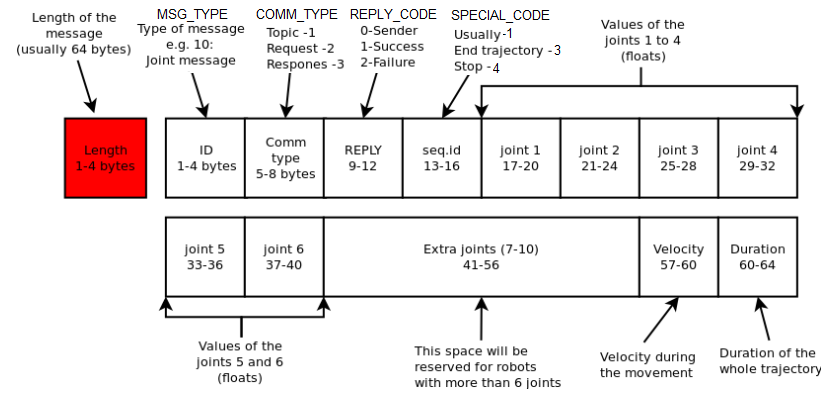
\includegraphics[width=1\textwidth]{Immagini/Message_Protocol}
	\caption{Struttura del messaggio scambiato tra client e server}
	\label{fig:MessageProtocol}
\end{figure}
\section{Client part}
\label{sec:Client}
Nella comunicazione socket che si va ad aprire, siamo in grado di individuare client e server custom per la gestione dei manipolatori ABB.

Le principali funzionalità che un client di questo tipo dovrebbe avere, sono quelle di andare a gestire lo stato corrente dei giunti del manipolatore, ricevendo le informazioni dal controller IRC5 Compact e rielaborandole secondo le necessità.

Il primo step è sicuramente quello di andare ad avviare due packages che si trovano all'interno della nostra applicazione:
\begin{itemize}
	\item abb\_driver
	\item unibg\_robot\_controller
\end{itemize}
Infatti tutto il software ROS, come accennato in precedenza, presenta un'organizzazione a package: nello specifico, un package ROS rappresenta una collezione di file, genericamente sia file eseguibili che di supporto, utilizzati per scopi specifici ed organizzati all'interno di una struttura gerarchica ben precisa (si troveranno sempre due file specifici: il \emph{manifesto} con estensione .xml ed un file \emph{CMakeList}, un file .txt da fornire come input al CMake build per costruire la struttura software dei package).
Nello specifico dei due package sopra riportati, andiamo a lanciare solamente due parti specifiche, che poi andranno ad avviare l'intero insieme dei nodi. Queste parti sono:
\begin{description}
	\item[robot\_interface.launch:] questo file .launch fornisce gli strumenti necessari per andare ad aprire l'effettiva comunicazione socket tra il sistema ROS e il manipolatore ABB, utilizzando il protocollo standard di ROS Industrial spiegato nel paragrafo~\vref{text:MessaggeProtocol}. Possiamo infatti passare a questo particolare tipo di file alcune informazioni chiave, quali l'indirizzo IP del robot da gestire unitamente al file URDF necessario per definire la geometria del manipolatore in uso.
	
	Utilizzando il comando \emph{roslaunch} si è in grado di lanciare files con estensione .launch, permettendo di andare ad avviare più nodi contemporaneamente, quali:
	\begin{description}
		\item[robot\_state:] esso si connette al modulo di programma \emph{State\_Server} caricato a bordo del controller, ed è responsabile della pubblicazione dello stato corrente del robot e del valore in gradi dei 6 giunti del manipolatore. 
		\item[motion\_download\_interface:] gestisce la movimentazione del robot, spedendo al controllore IRC5 Compact punti formanti una traiettoria.
		\item[joint\_trajectory\_action:] si tratta di un nodo che permette di fornire al controller i punti che il manipolatore deve raggiungere (figura~\vref{fig:joint-trajectory-action}) e toccare per seguire una specifica traiettoria, segnalando allo stesso tempo la corretta esecuzione e il raggiungimento dell'obbiettivo.
		
		Questo nodo presenta inoltre la possibilità di imporre dei vincoli alla movimentazione, potendo interrompere l'esecuzione della traiettoria stessa nel momento in cui i vincoli risultano essere violati.  
		\begin{figure}[h]
			\centering
			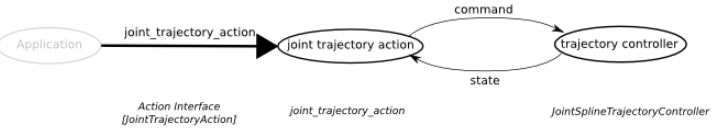
\includegraphics[width=1\textwidth]{Immagini/joint_trajectory_action}
			\caption{Funzionalità del nodo joint\_trajectory\_action}
			\label{fig:joint-trajectory-action}
		\end{figure}
	\end{description} 
	\item[unibg\_simple\_move\_node:] nel punto precedente, l'avvio del file robot\_interface.launch ci ha permesso di avviare contemporaneamente più nodi. In questo caso, utilizzando il comando \emph{rosrun}, andiamo ad avviare un singolo nodo ROS, il quale permette di andare a pubblicare messaggi di tipo \emph{control\_msgs::FollowJointTrajectoryActionGoal} sul topic \emph{joint\_trajectory\_action/goal}.
	
	Nello specifico, il messaggio che viene pubblicato sul topic ha un a struttura ben precisa, la quale è formata da:
	\begin{description}
		\item[std\_msgs/Header header:] esso è utilizzato per trasmettere l'informazione in merito al timestamp della comunicazione unitamente all'identificativo del tipo di sistema di riferimento utilizzato per definire le coordinate (\emph{no\_frame} oppure \emph{global\_frame}).
		\item[actionlib\_msgs/GoalID\ goal\_id:] esso contiene un timestamp che rappresenta l'istante in cui è stata richiesta una certa coordinata; questo istante è utilizzato dal server, posto sul controller, quando tenta di andare ad annullare tutte le traiettorie richieste prima di un certo timeout.
		Oltre al timestamp è presente un campo identificativo univoco che permette di associare un certo feedback ad una specifica traiettoria.
		\item[control\_msgs/FollowJointTrajectoryGoal\ goal:] in questo campo del messaggio pubblicato dal nostro nodo unibg\_simple\_move\_node si vanno a definire tra parametri importanti:
		\begin{description}
			\item \emph{goal\_time\_tolerance}: indica la tollerenza temporale entro il quale si impone il raggiungimento del punto stabilito
			\item \emph{path\_tolerance e goal\_tolerance}: se la misura dei parametri di joint di velocità, poisizione e accelerazione cade fuori dal range di tolleranza, la traiettoria è abortita.
			\item \emph{trajectory\_msgs/JointTrajectory trajectory}: qui è contenuta l'informazione più importante, ovvero quella che riguarda i punti che vanno a comporre la traiettoria, unitamente al nome dei joint.
		\end{description}		
	\end{description}
	L'informazione contenuta nel messaggio denominato precedentemente come \emph{goal} sarà quindi poi pubblicato dal nostro nodo, tramite i comandi mostrati nel listato~\vref{Code:TopicsPub}.
	\begin{lstlisting}[style=Matlab-editor,caption=Pubblicazione messagio \emph{trajectory} di esempio nel topic corrispondente,captionpos=b,label={Code:TopicsPub}, basicstyle=\tiny\ttfamily,frame=trBL]
		ros::Publisher pub_joint_action = n.advertise<control_msgs::FollowJointTrajectoryActionGoal>("joint_trajectory_action/goal", 1);
		control_msgs::FollowJointTrajectoryActionGoal goal;

		goal.goal.trajectory.header.stamp = ros::Time::now() + ros::Duration(1.0);
		int ind = 0;
		goal.goal.trajectory.points[ind].positions.resize(6);
		goal.goal.trajectory.points[ind].positions[0] = -1.3963;
		goal.goal.trajectory.points[ind].positions[1] = 0.65;
		goal.goal.trajectory.points[ind].positions[2] = 0.5461;
		goal.goal.trajectory.points[ind].positions[3] = 0.0;
		goal.goal.trajectory.points[ind].positions[4] = 0.3747;
		goal.goal.trajectory.points[ind].positions[5] = 0.0;
		goal.goal.trajectory.points[ind].time_from_start = ros::Duration(5.0);
	\end{lstlisting}
\end{description}
Gli elementi caratterizzanti il sistema sono però i topic: infatti, una volta avviati i nodi (per mezzo dei comandi \emph{rosrun} e \emph{roslaunch}), nascono alcuni topic specifici, i quali possono andare a scambiare solamente determinate tipologie di messaggi (per la struttura dei messaggi legati ai singoli topic fare riferimento a \cite{online:ROS-api}). I topic che si creano, come si può vedere nella figura~\vref{fig:rosgraph} sono:
\begin{itemize}
	\item /feedback\_states
	\item /joint\_path\_command
	\item /joint\_trajectory\_action/cancel
	\item /joint\_trajectory\_action/feedback
	\item /joint\_trajectory\_action/goal
	\item /joint\_trajectory\_action/result
	\item /joint\_trajectory\_action/status
	\item  /robot\_status
\end{itemize}
\begin{figure}
	\centering
	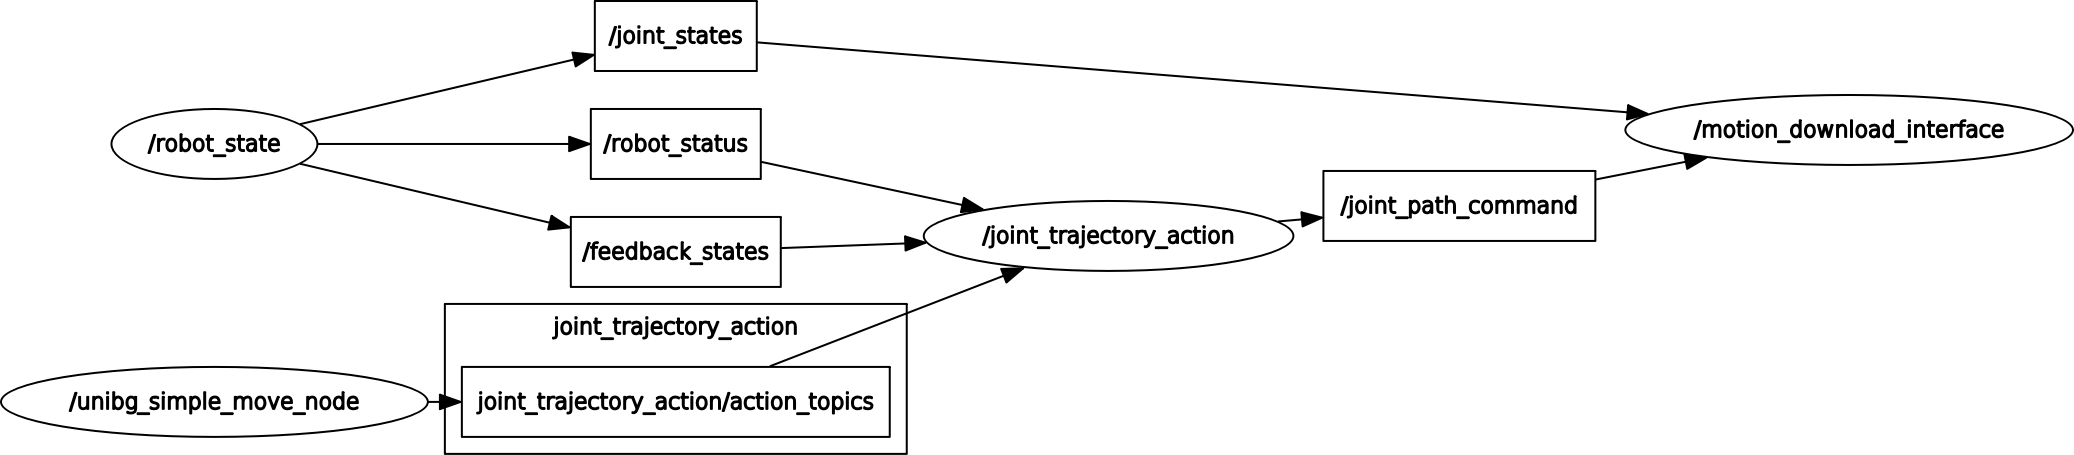
\includegraphics[width=1.3\textwidth]{Immagini/rosgraph}
	\caption{Grafo delle dipendenze tra topics e nodi}
	\label{fig:rosgraph}
\end{figure}
\section{Architettura ABB ROS Server}
Come visto in precedenza (capitolo~\vref{text:pubsub}), il fulcro del controllo tramite ROS sta proprio in un continuo scambio di messaggi sul modello \emph{publisher-subscriber}: essa può essere quindi considerata come una struttura client-server, dove il client è rappresentato da un insieme di nodi \emph{ROS} in grado di pubblicare particolari tipologie di messaggi (sezione~\vref{sec:Client}). 

Il server è invece rappresentato, per forza di cose, dal controllore IRC5 Compact, il quale deve essere in grado di andare a ricevere le informazioni necessarie per gestire la traiettoria del robot, per mezzo dell'instaurazione di una comunicazione tramite socket.

Per poter andare a configurare il controllore è necessario fare riferimento ancora all'ambito di programmazione \emph{RobotStudio}: in questo caso però, una volta configurato il codice RAPID e caricato a bordo del controller stesso, non avremo più bisogno di modificare la struttura, poichè la traiettoria verrà gestita direttamente dall'ambiente ROS, ottenendo il comportamento dinamico desiderato.
Nello specifico risultano essere necessari tre task: 
\begin{itemize}
	\item T\_ROB1
	\item ROS\_StateServer
	\item ROS\_MotionServer
\end{itemize}
\begin{figure}
	\centering
	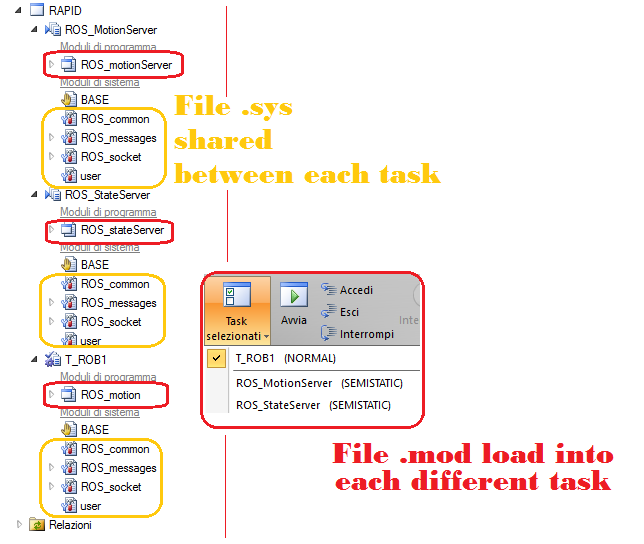
\includegraphics[width=0.75\textwidth]{Immagini/ParallelTask_VirtualController}
	\caption{Struttura multitasking del server ROS implementato in codice RAPID}
	\label{fig:ParallelTask}
\end{figure}

La struttura principale della nostra applicazione \emph{RAPID} è quindi formata da più task, i quali procedono la loro esecuzione in parallelo, a partire dal momento in cui l'esecuzione inzia, fino ad un tempo potenzialmente infinito(a meno di errori presenti all'interno del codice stesso): non tutti e tre i task hanno però lo stesso peso e le stesse funzionalità, come si può vedere nella figura~\vref{fig:TaskConfiguration}. 
\label{text:TROB1}

Il task T\_ROB1 rappresenta l'unico task che può andare gestire direttamente la movimentazione del manipolatore tramite istruzioni di movimento, essendo configurato come \emph{Motion Task}: per le proprietà della programmazione in RobotStudio, qualsiasi task impostato come task di movimento, deve essere di tipo NORMAL, ovvero deve poter essere eseguito in primo piano. Questo implica che, per andare a movimentare il manipolatore, è necessario, come primo step, andare ad attivare questo task.

ROS\_StateServer e ROS\_MotionServer sono invece configurati come task SEMISTATIC: si tratta quindi di task in \emph{background}, il cui funzionamento non può essere controllato, ovvero vengono eseguiti automaticamente nel momento in cui il controllore viene avviato.
\begin{figure}[h]
	\centering
	\includegraphics[width=0.75\textwidth]{Immagini/Task_Configuration}
	\caption{Configurazioni dei task del ROSserver}
	\label{fig:TaskConfiguration}
\end{figure}

Questa rappresenta però la struttura "statica" dei task che vanno a comporre il server ROS (sezione~\vref{sec:Server}): in ognuno di esso è necessario andare a caricare moduli di programma contenenti le istruzioni RAPID da eseguire. Si tratta dei moduli \emph{ROS StateServer.mod, ROS MotionServer.mod e TROB\_1}, ai quali vanno aggiunti anche i moduli di sistema \emph{ROS common.sys, ROS socket.sys e ROS messages.sys}, i quali risultano essere condivisi tra tutti i task. 

La parte "dinamica" dell'intera applicazione risulta essere invece sviluppata e costrutita in ambiente Unix, grazie alle funzionalità offerte dal sistema operativo ROS (sezione~\vref{sec:Client}).




\section{Server part}
\label{sec:Server}
\subsection{ROS\_MotionServer}
Essendo che il modulo caricato all'interno del task omonimo si trova in continua esecuzione, una volta che viene stabilita la connessione socket tra client e server, esso inizia a ricevere messaggi contenenti i punti formanti le traiettorie inviate dal client ROS, come si può vedere nel listato:
\begin{lstlisting}[style=Matlab-editor,caption=Ricezione delle traiettorie con relativo controllo d'integrità,captionpos=b,label={Code:ROSMotionServer},basicstyle=\scriptsize\ttfamily,frame=trBL]
	LOCAL CONST num server_port := 11000;
	
	LOCAL VAR socketdev server_socket;
	LOCAL VAR socketdev client_socket;
	LOCAL VAR ROS_joint_trajectory_pt trajectory{MAX_TRAJ_LENGTH};
	LOCAL VAR num trajectory_size;
	
	PROC main()
		VAR ROS_msg_joint_traj_pt message;
		
		TPWrite "MotionServer: Waiting for connection.";
		ROS_init_socket server_socket, server_port;
		ROS_wait_for_client server_socket, client_socket;
		
		WHILE ( true ) DO
			ROS_receive_msg_joint_traj_pt client_socket, message;
			trajectory_pt_callback message;
		ENDWHILE
		
	ERROR (ERR_SOCK_TIMEOUT, ERR_SOCK_CLOSED)
		IF (ERRNO=ERR_SOCK_TIMEOUT) OR (ERRNO=ERR_SOCK_CLOSED) THEN
			SkipWarn;  
			ErrWrite \W, "ROS MotionServer disconnect", "Connection lost.  Resetting socket.";
			ExitCycle;  % restart program
		ELSE
			TRYNEXT;
		ENDIF
	UNDO
		IF (SocketGetStatus(client_socket) <> SOCKET_CLOSED) SocketClose client_socket;
		IF (SocketGetStatus(server_socket) <> SOCKET_CLOSED) SocketClose server_socket;
	ENDPROC
\end{lstlisting}

Nella ricezione dei punti che compongono una data traiettoria è però importante andare a distinguerne due: il punto iniziale e il punto finale.

Quindi, unitamente alla ricezione del messaggio per mezzo della procedura ROS\_receive\_msg\_joint\_traj\_pt condivisa tramite il modulo di sistema ROS\_messages, si va a richiamare la procedura locale trajectory\_pt\_callback la quale, con una semplice struttura switch case effettuata sul campo \emph{sequence\_id} del messaggio, permette di andare a verificare che tipo di punto stiamo andando ad analizzare.
\begin{lstlisting}[style=Matlab-editor,caption=Struttura che permette di riconoscere la natura del punto da aggiungere alla traiettoria in esame,captionpos=b,label={Code:ROSMotionServer2},basicstyle=\scriptsize\ttfamily,frame=trBL]
	TEST message.sequence_id
		CASE ROS_TRAJECTORY_START_DOWNLOAD:
			TPWrite "Traj START received";
			trajectory_size := 0;                 % Reset  della trajectory size
			add_traj_pt point;              
		CASE ROS_TRAJECTORY_END:
			TPWrite "Traj END received";
			add_traj_pt point;                    
			activate_trajectory;
		CASE ROS_TRAJECTORY_STOP:
			TPWrite "Traj STOP received";
			trajectory_size := 0;  %
			activate_trajectory;
			StopMove; ClearPath; StartMove; 
		DEFAULT:
			add_traj_pt point;            
	ENDTEST
\end{lstlisting}


\subsection{ROS\_StateServer}
Il compito principale del modulo di programma contenuto in questo task, è quello di andare ad inviare messaggi broadcast contenenti informazioni e dati in merito alla posizione dei giunti.
In particolar modo la funzionalità di questo modulo, il quale rimane in esecuzione continuamente in background, è molto importante: esso permette, una volta stabilita la connessione socket, di inviare al client, ad un determinato rate (\emph{update\_rate}), la posizione corrente dei 6 giunti. 

Si chiude così l'anello di retroazione, tramite un feedback che risulta essere molto importante per quelle applicazioni in cui è necessaria un'elevata precisione nella movimentazione.  
\begin{lstlisting}[style=Matlab-editor,caption=Feedback continuo della posizione del manipolatore,captionpos=b,label={Code:ContinuosFeedBack},basicstyle=\scriptsize\ttfamily,frame=trBL]
	LOCAL CONST num server_port := 11002;
	LOCAL CONST num update_rate := 0.10;  % broadcast rate (sec)
	
	LOCAL VAR socketdev server_socket;
	LOCAL VAR socketdev client_socket;
	
	PROC main()
	
		TPWrite "StateServer: Waiting for connection.";
		ROS_init_socket server_socket, server_port;
		ROS_wait_for_client server_socket, client_socket;
		
		% Spedizione con periodo pari a update_rate del valore attuale dei joint
		WHILE (TRUE) DO
		send_joints;
		WaitTime update_rate;
		ENDWHILE
\end{lstlisting}

\subsection{ROS\_Motion: effettiva movimentazione del manipolatore}
In questo task, all'interno del modulo caricatovi a bordo, come anticipato nel paragrafo~\vref{text:TROB1}, avremo le effettive istruzioni che vanno a mettere in movimento il robot, essendo che esso è caricato all'interno del task T\_ROB1, il quale è definito come l'unico \emph{Motion Task}. 

Il concetto base è che dall'ambiente ROS, più nello specifico dal modulo ROS\_motion\_server.mod, si ricevono un insieme di punti (o \emph{targets}), i quali vanno a comporre la traiettoria che il manipolatore dovrà andare a seguire.

In sostanza si scandisce con un ciclo tutta la lista dei target, la cui lettura è eseguita nella soubrutine \emph{init trajectory()}, tramite l'utilizzo di un lock sulla lettura cosicchè nessuno vada sovrascrivere la traiettoria mentre se ne sta effettuando l'acquisizione.
\begin{lstlisting}[style=Matlab-editor,caption=Movimentazione effettiva del manipolatore,captionpos=b,label={Code:ROSMotion}, basicstyle=\scriptsize\ttfamily,frame=trBL]

	% Il server e' settato per ricevere una serie di target e poi andare ad eseguire un insieme conosciuto di posizioni, non dando la possibilita' di aggiungere target "on-the-fly"
	
	LOCAL VAR ROS_joint_trajectory_pt trajectory{MAX_TRAJ_LENGTH};
	LOCAL VAR num trajectory_size := 0;
	LOCAL VAR intnum intr_new_trajectory;
	
	PROC main()
		VAR num current_index;
		VAR jointtarget target;
		VAR speeddata move_speed := v10;  % velocita' di default
		VAR zonedata stop_mode;
		VAR bool skip_move;
				
		WHILE true DO
			% La variabile "ROS_new_trajectory" e' una variabile di tipo "PERSistent bool", la quale permette di mantenere l'ultimo valore salvato, anche in caso di interruzione dell'esecuzione, ed e' necessaria per segnalare se e' disponibile o meno una nuova traiettoria
			IF (ROS_new_trajectory)
				% Acquisizione, con lock, della traiettoria
				init_trajectory;
			
			% Analizzo i punti componenti la traiettoria
			IF (trajectory_size > 0) THEN
				FOR current_index FROM 1 TO trajectory_size DO
					%Acquisisco i valori in gradi dei 6 giunti
					target.robax := trajectory{current_index}.joint_pos;
					
					% Se il primo punto e' vicino (entro i limiti di tolleranza) al punto da raggiungere, allora devo saltare questo target
					skip_move := (current_index = 1) AND is_near(target.robax, 0.1);
					IF (current_index = trajectory_size) 
						stop_mode := fine;  % stop at path end
					
					%=====================================================
					% Effettiva esecuzione del movimento
					IF (NOT skip_move)
						MoveAbsJ target, move_speed, \T:=trajectory{current_index}.duration, stop_mode, tool0;
					%=====================================================
				ENDFOR
				
				trajectory_size := 0;  % movimentazione eseguita
			ENDIF
			
			WaitTime 0.05; 
		ENDWHILE
		
		ERROR
			ErrWrite \W, "Motion Error", "Error executing motion.  Aborting trajectory.";
			abort_trajectory;
	ENDPROC
\end{lstlisting}

\subsection{ROS\_Socket: apertura della connessione socket lato server}
Nell'archietettura del server, ROS\_socket rappresenta un modulo di sistema (vedi~\vref{text:SysModule}): esso quindi risulta essere condiviso tra tutti i task, i quali hanno quindi la possibilità di richiamare le funzioni che vi sono al suo interno. 
Nello specifico, il modulo di sistema in esame, contiene 4 routine che permettono di gestire l'interazione con il socket, le quali sono:
\begin{description}
	\item[ROS\_init\_socket:] in questa funzione si vanno a definire i parametri della connessione, quali l'indirizzo IP e il numero della porta, e successivamente la si va a creare, associandolo alla variabile di tipo \emph{socketdev} fornita in ingresso alla funzione.
	\begin{lstlisting}[style=Matlab-editor,caption=Analisi funzionamento routine ROS-init-socket ,captionpos=b,label={Code:ROSinitsocket}, basicstyle=\scriptsize\ttfamily,frame=trBL]
		% SocketGetStatus e' un istruzione che restituisce lo stato corrente di un socket, il quale puo' essere:
		 - SOCKET_CREATED
		 - SOCKET_CONNECTED
		 - SOCKET_BOUND
		 - SOCKET_LISTENING
		 - SOCKET_CLOSED
		% Se non esiste alcuna connessione socket la vado a creare 
		IF (SocketGetStatus(server_socket) = SOCKET_CLOSED) SocketCreate server_socket;
		
		% Se il socket e' stato gia' creato allora associo al socket stesso l'indirizzo ip specificato del server e il numero della  sua porta. Da evidenziare il fatto che l'indirizzo del server e' ottenuto automaticamente, come indirizzo del controller tramite l'istruzione GetSysInfo
		
		IF (SocketGetStatus(server_socket) = SOCKET_CREATED) SocketBind server_socket, GetSysInfo(\LanIp), port;
		
		% Qui il controller, che lavora come un server, inizia effettivamente ad ascoltare e ricevere le comunicazioni in ingresso
		IF (SocketGetStatus(server_socket) = SOCKET_BOUND) SocketListen server_socket;
	\end{lstlisting}
\end{description}
\begin{description}
	\item[ROS\_wait\_for\_client:] con questa funzione si va a stabilire l'effettiva connessione tra client e server della comunicazione socket.
	
	Nello specifico in questa funzione, si ha una gestione della connessione che possiamo definire "temporizzata": infatti, tra i parametri di input è presente la variabile numerica facoltativa \emph{wait\_time} che permette di specificare la quantità massima di tempo riservata all'esecuzione del programma per l'attesa di connessioni in arrivo. Nel caso in cui questo tempo scada, senza che giunga alcuna connessione in ingresso, si andrà a generare un errore (ERR\_SOCK\_TIMEOUT) che poi verrà ad essere gestito.
	\begin{lstlisting}[style=Matlab-editor,caption=Analisi funzionamento routine ROS-wait-for-client,captionpos=b,label={Code:ROSwaitforclient}, basicstyle=\scriptsize\ttfamily,frame=trBL]	
		VAR string client_ip;
		VAR num time_val := WAIT_MAX; 		

		% Essendo il parametro wait\_time facoltativo, devo verificare che sia presente
		IF Present(wait_time) time_val := wait_time;
		
		IF (SocketGetStatus(client_socket) <> SOCKET_CLOSED) SocketClose client_socket;
		WaitUntil (SocketGetStatus(client_socket) = SOCKET_CLOSED);
		
		% L'istruzione SocketAccept, utilizzabile solamente lato server, permette di andare ad accettare una connessione in arrivo: una volta accettata la connessione, lo stato del socket diventa di SOCKET_LISTENING
		
		SocketAccept server_socket, client_socket, \ClientAddress:=client_ip, \Time:=time_val;
		TPWrite "Client at "+client_ip+" connected.";
	\end{lstlisting}
\end{description}
\begin{description}
	\item[ROS\_receive\_msg:] questo routine è prevalentemente utilizzata dal modulo di sistema \emph{ROS\_messages.sys}, il quale se ne serve per andare a salvare momentaneamente in una variabile "buffer" i dati ricevuti dalla comunicazione socket, tramite l'utilizzo dell'istruzione \emph{UnpackRawBytes}, necessaria per raggruppare il contenuto di un contenitore di tipo rawbytes.
	
	Successivamente tutti i dati ricevuti vengono inseriti all'interno della variabile message, che è quindi pronta per la conversione e per essere elaborata.
	\item[ROS\_send\_msg:] questa routine riceve la posizione corrente dei joint del manipolatore, all'interno di una variabile di tipo \emph{ROS\_msg}. I dati, in formato raw bytes, sono analizzati, riuniti secondo la struttura del messaggio del protocollo (sezione~\vref{text:MessaggeProtocol}) ed infine vengono spediti attraverso il socket. 

	Si tratta quindi di una comunicazione di feedback del server verso il client: in sostanza permette al codice sviluppato in ROS di verificare la correttezza della movimentazione.
\end{description}
\subsection{ROS\_messages}
In questo modulo di sistema, si vanno a creare 4 tipologie di variabili utilizzate per contenere i dati inerenti alle traiettorie e ai punti che le compongono. Sono presenti inoltre 2 procedure che permettono di operare una trasformazione e uno scambio di messaggi.
\begin{description}
	\item[ROS\_receive\_msg\_joint\_traj\_pt:] in questa procedura si va a convertire il messaggio \emph{raw\_message}, mandato dal client, nella variabile \emph{message}.
	Si tratta di variabili che hanno sostanzialmente una struttura diversa: \emph{raw\_message} è una variabile di tipo ROS\_msg la cui struttura è riporta nel listato seguente, mentre \emph{message} è la variabile che viene effettivamente utilizzata per effettuare la movimentazione desiderata, ed essa è di tipo ROS\_msg\_joint\_traj\_pt, la cui struttura è invece riportata nel listato~\vref{Code:RecordROSmsgjointtrajpt} e nella figura~\vref{fig:MessageProtocol}.
	\begin{lstlisting}[style=Matlab-editor,caption=Campi caratterizzanti il tipo di variabili ROS-msg,captionpos=b,label={Code:RecordROSmsg}, basicstyle=\scriptsize\ttfamily,frame=trBL]	
		RECORD ROS_msg
			num msg_type;
			num comm_type;
			num reply_code;
			rawbytes data;
		ENDRECORD
	\end{lstlisting}
	\begin{lstlisting}[style=Matlab-editor,caption=Campi caratterizzanti il tipo di variabili ROS-msg-joint-traj-pt,captionpos=b,label={Code:RecordROSmsgjointtrajpt}, basicstyle=\scriptsize\ttfamily,frame=trBL]	
		RECORD ROS_msg_joint_traj_pt
			num msg_type;
			num comm_type;
			num reply_code;
			num sequence_id;
			robjoint joints;  % in gradi
			num velocity;
			num duration;
		ENDRECORD
	\end{lstlisting}
	
	Il trasferimento effettivo da una forma di messaggio all'altra, che altro non è che il cuore di questa procedura, unitamente alla conversione in gradi, è riportato nel codice~\vref{Code:Unpack}.
	\begin{lstlisting}[style=Matlab-editor,caption=Unpacking del messaggio ricevuto dal client,captionpos=b,label={Code:Unpack}, basicstyle=\tiny\ttfamily,frame=trBL]	
		UnpackRawBytes raw_message.data, 1, message.sequence_id, \IntX:=DINT;
		UnpackRawBytes raw_message.data, 5, message.joints.rax_1, \Float4;
		UnpackRawBytes raw_message.data, 9, message.joints.rax_2, \Float4;
		UnpackRawBytes raw_message.data, 13, message.joints.rax_3, \Float4;
		UnpackRawBytes raw_message.data, 17, message.joints.rax_4, \Float4;
		UnpackRawBytes raw_message.data, 21, message.joints.rax_5, \Float4;
		UnpackRawBytes raw_message.data, 25, message.joints.rax_6, \Float4;
		% Skip bytes 29-44.  UNUSED.  Reserved for Joints 7-10.
		UnpackRawBytes raw_message.data, 29+(ROS_MSG_MAX_JOINTS-6)*4, message.velocity, \Float4;
		UnpackRawBytes raw_message.data, 33+(ROS_MSG_MAX_JOINTS-6)*4, message.duration, \Float4;
		% Convert data from ROS units to ABB units
		message.joints := rad2deg_robjoint(message.joints);
	\end{lstlisting}
	\item[ROS\_send\_msg\_joint\_data:] in questa routine invece si va ad effettuare un'operazione nella direzione opposto di quella compiuta all'interno della procedura ROS\_receive\_msg\_joint\_traj\_pt. Si ricostruiscee quindi la struttura del messaggio adatta per essere inviata al client, come feedback.   
	\begin{lstlisting}[style=Matlab-editor,caption=Packing del messaggio per spedizione verso il client come mezzo di feedback,captionpos=b,label={Code:Pack}, basicstyle=\tiny\ttfamily,frame=trBL]	
		PackRawBytes message.sequence_id, raw_message.data,  1, \IntX:=DINT;
		PackRawBytes ROS_joints.rax_1,    raw_message.data,  5, \Float4;
		PackRawBytes ROS_joints.rax_2,    raw_message.data,  9, \Float4;
		PackRawBytes ROS_joints.rax_3,    raw_message.data, 13, \Float4;
		PackRawBytes ROS_joints.rax_4,    raw_message.data, 17, \Float4;
		PackRawBytes ROS_joints.rax_5,    raw_message.data, 21, \Float4;
		PackRawBytes ROS_joints.rax_6,    raw_message.data, 25, \Float4;
		FOR i FROM 1 TO ROS_MSG_MAX_JOINTS-6 DO   % Insert placeholders for joints 7-10 (message expects 10 joints)
		PackRawBytes 0,               raw_message.data, 25+i*4, \Float4;
		ENDFOR
		
		ROS_send_msg client_socket, raw_message;
	\end{lstlisting}
\end{description}
%=================================================================================
	\chapter{Estensioni future}
	Lo studio condotto in questa sede ha permesso di andare a fornire il \emph{know-how} necessario per poter avviare progetti di ricerca riguardanti questa tipologia di manipolatori: nello specifico siamo riusciti ad avere un quadro più completo di quelle che possono essere le possibili tecniche di gestione e controllo del movimento.
	Sicuramente, con il tempo avuto a disposizione, ci siamo trovati di fronte a prendere delle scelte: il compito dunque di questo percorso è stato proprio quello di andare ad aprire la strada per lavori/progetti futuri. 
	Nello specifico, è stato sempre tenuto presente che, il primissimo step futuro da eseguire, sarà quello di andare a creare una movimentazione autonoma del robot, per mezzo dell'utilizzo di  sensori visuali, quali telecamere, webcam oppure sensori visuali 3D.
	Contemporaneamente all'introduzione di una gestione autonoma del manipolatore, bisognerà andare a valutare le informazioni fornite come feedback dalla cinematica inversa: sarà infatti necessario andare a discriminare le soluzioni valide da quelle che invece non sono in grado di andare a rispettare vincoli di tipo fisico. Questo potrebbe essere possibile grazie all'utilizzo di nuovi algoritmi di controllo, unitamente ad una stesura di codice completamente orientato verso l'ambiente Matlab.
	%====================================================================
	\backmatter
	\nocite{*}
	\printbibliography
\end{document}

%==================================================================